\chapter{Horizontal Composition: Systems Built from Many Protocols}
\label{chap:disel}

\newcounter{tagz}

% colors
\definecolor{shadecolor}{gray}{1.00}
\definecolor{darkgray}{gray}{0.30}
\definecolor{violet}{rgb}{0.56, 0.0, 1.0}
\definecolor{forestgreen}{rgb}{0.13, 0.55, 0.13}

% Col language definition
\lstdefinelanguage{Coq} {
mathescape=true,						
texcl=false,
morekeywords=[1]{
  Add,
  All,
  Arguments,
  Axiom,
  Bind,
  Canonical,
  Check,
  Close,
  CoFixpoint,
  CoInductive,
  Coercion,
  Contextual,
  Corollary,
  Defined,
  Definition,
  Delimit,
  End,
  Example,
  Export,
  Fact,
  Fixpoint,
  Goal,
  Graph,
  Hint,
  Hypotheses,
  Hypothesis,
  Implicit,
  Implicits,
  Import,
  Inductive,
  Lemma,
  Let,
  Local,
  Locate,
  Ltac,
  Maximal
  Module,
  Morphism,
  Next,
  Notation,
  Obligation,
  Open,
  Parameter,
  Parameters,
  Prenex,
  Print,
  Printing,
  Program,
  Projections,
  Proof,
  Proposition,
  Qed,
  Record,
  Relation,
  Remark,
  Require,
  Reserved,
  Resolve,
  Rewrite,
  Save,
  Scope,
  Search,
  Section,
  Show,
  Strict,
  Structure,
  Tactic,
  Theorem,
  Unset,
  Variable,
  Variables,
  View,
  inside,
  outside
},
morekeywords=[2]{
  as,
  cofix,
  else,
  end,
  exists,
  exists2,
  fix,
  for,
  forall,
  fun,
  if,
  in,
  is,
  let,
  match,
  nosimpl,
  of,
  return,
  struct,
  then,
  vfun,
  with
},
morekeywords=[3]{Type, Prop, Set, True, False},
morekeywords=[4]{
  after,
  apply,
  assert,
  auto,
  bool_congr,
  case,
  change,
  clear,
  compute,
  congr,
  cut,
  cutrewrite,
  destruct,
  elim,
  field,
  fold,
  generalize,
  have,
  heval, 
  hnf,
  induction,
  injection,
  intro,
  intros,
  intuition,
  inversion,
  left,
  loss,
  move,
  nat_congr,
  nat_norm,
  pattern,
  pose,
  refine,
  rename,
  replace,
  revert,
  rewrite,
  right,
  ring,
  set,
  simpl,
  split,
  suff,
  suffices,
  symmetry,
  transitivity,
  trivial,
  unfold,
  unlock,
  using,
  without,
  wlog,
  autorewrite
},        
morekeywords=[5]{
  assumption,
  by,
  contradiction,
  done,
  exact,
  lia,
  gappa,
  omega,
  reflexivity,
  romega,
  solve,
  tauto,
  discriminate,
  unsat
},
morecomment=[s]{(*}{*)},
morekeywords=[6]{do, first, try, idtac, repeat},
showstringspaces=false,
morestring=[b]",
% Size of tabulations
tabsize=3,							
% Enables ASCII chars 128 to 255
extendedchars=true,  		 		
% Case sensitivity
sensitive=true, 
% Automatic breaking of long lines
breaklines=false,
% Default style fors listings
%basicstyle=\scriptsize\ttfamily,
basicstyle=\footnotesize\ttfamily,
% Position of captions is bottom
captionpos=b,							
% Full flexible columns 
columns=[l]fullflexible,
% Style for (listings') identifiers
identifierstyle={\color{black}},
% Style for declaration keywords
keywordstyle=[1]{\color{violet}},
% Style for gallina keywords
keywordstyle=[2]{\color{forestgreen}},
% Style for sorts keywords
keywordstyle=[3]{\color{forestgreen}},
% Style for tactics keywords
keywordstyle=[4]{\color{blue}},
% Style for terminators keywords
keywordstyle=[5]{\color{red}},
%Style for iterators
keywordstyle=[6]{\color{violet}},
% Style for strings
stringstyle=,
% Style for comments
commentstyle=\it\ttfamily\color{brown},
% Style for lines numbering
numberstyle=\tiny,
literate={\\/}{{$\vee$}}1
         {/\\}{{$\wedge$}}1
         {:->}{{$\mapsto~$\!}}1
         {\\->}{{$\mapsto~$\!}}1
         {<--}{{$\asgn~$}}1
         {\\in}{{$\in~$}}1
         {++}{{$+\!+\!~$}}1
         {->}{{$\to~$}}1
         {forall}{{$\forall~$}}1
         {exists}{{$\exists~$}}1
         {=>}{{$\Rightarrow~$}}1
         {\\+}{{$\!\join\!~$}}1
}

\lstdefinestyle{Coq}{language=Coq}
%\lstset{style=Coq}
\hyphenation{Dist-Algo}
\hyphenation{Ssref-lect}

% Colors

\definecolor{shadecolor}{gray}{1.00}
\definecolor{ddarkgray}{gray}{0.75}
\definecolor{darkgray}{gray}{0.30}
\definecolor{light-gray}{gray}{0.87}
\newcommand{\whitebox}[1]{\colorbox{white}{#1}}
\newcommand{\graybox}[1]{\colorbox{light-gray}{#1}}
\newcommand{\darkgraybox}[1]{\colorbox{ddarkgray}{#1}}
\newcommand{\gbm}[1]{\graybox{${#1}$}}
\newcommand{\Inv}{\text{\textsc{Inv}}}
\newcommand{\TPCInv}{\text{\textsc{TPCInv}}}

\newcommand{\fstar}{\text{F}^{\star}}
%\newcommand{\etc}{\emph{etc}}
%\newcommand{\ie}{\emph{i.e.}\xspace}
\newcommand{\Ie}{\emph{I.e.}\xspace}
%\newcommand{\eg}{\emph{e.g.}\xspace}
\newcommand{\Eg}{\emph{E.g.}\xspace}
\newcommand{\vs}{\emph{vs.}\xspace}
%\newcommand{\etal}{{et~al.}\xspace}
\newcommand{\adhoc}{\emph{ad hoc}\xspace}
\newcommand{\viz}{\emph{viz.}\xspace}
\newcommand{\dom}[1]{\mathsf{dom}(#1)}
\newcommand{\aka}{\textit{a.k.a.}\xspace}
\newcommand{\cf}{\textit{cf.}\xspace}
\newcommand{\wrt}{\emph{wrt.}\xspace}
\newcommand{\Iff}{\emph{iff}\xspace}
\newcommand{\loef}{L\"{o}f}
\newcommand{\hord}{\sqsubseteq}
\newcommand{\many}[1]{\overline{#1}}

\newcommand{\FV}{\mathsf{FV}}


\newcommand{\ifext}[2]{\ifdefined\extflag{#1}\else{#2}\fi}
\newcommand{\ifcomm}[1]{\ifdefined\extcomm{#1}\else{}\fi}

%\theoremstyle{remark}
%\newtheorem{example}{Example}[section]

%\theoremstyle{definition}
%\newtheorem{definition}{Definition}[section]

% \theoremstyle{plain}
% \newtheorem{theorem}{Theorem}[section]
% \newtheorem{lemma}[theorem]{Lemma}
% \newtheorem{proposition}[theorem]{Proposition}
% \newtheorem{corollary}[theorem]{Corollary}

\newenvironment{proofsketch}{\trivlist\item[]\emph{Proof sketch}:}%
{\unskip\nobreak\hskip 1em plus 1fil\nobreak$\square$
\parfillskip=0pt%
\endtrivlist}


%\newcommand{\mute}[1]{\ifcomm{#1}}
\newcommand{\mute}[1]{{#1}}
\newcommand{\Rule}[1]{\textsc{#1}}

\newcommand{\ab}[1]{\widehat{#1}}
\newcommand{\This}[1]{\mathsf{this}~{#1}}
\newcommand{\tsend}{\mathsf{send}}
\newcommand{\treceive}{\mathsf{receive}}
\newcommand{\tskip}{\mathsf{skip}}

\newcommand{\withinvr}{{\sc WithInv}\xspace}
\newcommand{\from}{\mathit{from}}
\newcommand{\tto}{\mathit{to}}
\newcommand{\True}{\mathsf{True}}
\newcommand{\id}{\mathsf{id}}
\newcommand{\False}{\mathsf{False}}
\newcommand{\set}[1]{\left\{{#1}\right\}}
\newcommand{\angled}[1]{\langle{#1}\rangle}
\newcommand{\Type}{\mathcal{T}}


%% Specs
\newcommand{\specK}[1]{\ensuremath{\textcolor{blue}{\set{#1}}}}
\newcommand{\pre}[1]{\specK{{#1}}}
\newcommand{\post}[1]{\specK{{#1}}}
\newcommand{\psep}{\ast}

%% Protocols
\newcommand{\ppr}{\mathcal{P}}
\newcommand{\cpr}{\mathcal{C}}

%% State-space and Transitions
\newcommand{\treq}{\mathsf{Req}}
\newcommand{\tresp}{\mathsf{Resp}}
\newcommand{\acts}{\Send}
\newcommand{\actr}{\Recv}
\newcommand{\trans}[1]{\mathit{#1}}
\newcommand{\To}{\mathit{to}}
\newcommand{\Rs}{\mathit{rs}}
\newcommand{\From}{\mathit{from}}
\newcommand{\args}{\mathit{args}}
\newcommand{\ans}{\mathit{ans}}
\newcommand{\aand}{\wedge}
\newcommand{\aandb}{\&\!\!\!\&}
\newcommand{\oor}{\vee}
\newcommand{\body}{\mathit{body}}
\newcommand{\clients}{\overline{C}}
\newcommand{\servers}{\overline{S}}
\newcommand{\Send}{\mathsf{send}}
\newcommand{\Recv}{\mathsf{recv}}
\newcommand{\csend}[1]{\Send[#1]}
\newcommand{\creceive}[1]{\Recn[#1]}
\newcommand{\lab}{\ell}
\newcommand{\Some}{\mathsf{Some}}
\newcommand{\None}{\mathsf{None}}
\newcommand{\Truez}{\mathsf{True}}
\newcommand{\Falsez}{\mathsf{False}}

\makeatletter % allow us to mention @-commands
\def\arcr{\@arraycr}
\makeatother

\newcommand{\inject}{\ensuremath{\mathsf{inject}}\xspace{}}
\newcommand{\unitz}{\mathsf{unit}\xspace{}}
\newcommand{\letz}{\mathsf{{\bf let}}\xspace{}}
\newcommand{\inz}{\mathsf{{\bf in}}\xspace{}}
\newcommand{\retz}{\mathsf{{\bf return}}\xspace{}}
\newcommand{\readz}{\mathsf{{read}}\xspace{}}
\newcommand{\letrecz}{\mathsf{{\bf letrec}}\xspace{}}
\newcommand{\ifz}{\mathsf{{\bf if}}\xspace{}}
\newcommand{\thenz}{\mathsf{{\bf then}}\xspace{}}
\newcommand{\elsez}{\mathsf{{\bf else}}\xspace{}}
\newcommand{\Active}{\circ}
\newcommand{\res}{\mathsf{res}}
\newcommand{\Consumed}{\bullet}
\newcommand{\asgn}{\leftarrow}
\newcommand{\vd}[1] {\mathrel{\oset{~#1}{\vdash}}}
\newcommand{\blockr}{\mathsf{receive\_req}}
\newcommand{\blockresp}{\mathsf{receive\_resp}}
\newcommand{\osserver}{\mathsf{simple\_server}}
\newcommand{\dserver}{\mathsf{deleg\_server}}
\newcommand{\cclient}{\mathsf{compute}}
\newcommand{\bserver}{\mathsf{batch\_server}}
\newcommand{\mserver}{\mathsf{memo\_server}}
\newcommand{\num}[1]{{\text{{\scriptsize{#1}}}}}
\newcommand{\eqdef}{\triangleq}
\newcommand{\withinv}{\mathsf{WithInv}}
\newcommand{\serv}{\mathit{serv}}
\newcommand{\figsize}{\footnotesize}
\newcommand{\NHooked}{\mathsf{NotHooked}}
\newcommand{\NotHooked}[1]{\NHooked(#1)}
\newcommand{\HooksOk}{\mathsf{HooksOk}}
\newcommand{\AllHooksOk}[1]{\HooksOk(#1)}

% Fancy pointers
\makeatletter
\newcommand{\oset}[3][0ex]{%
  \mathrel{\mathop{#3}\limits^{
    \vbox to#1{\kern-2\ex@
    \hbox{$\scriptstyle#2$}\vss}}}}
\makeatother

\newcommand{\ppts}[1]{\mathrel{\oset{#1}{\rightarrowtail}}}
\newcommand{\pmap}{\mathrel{\overset{\text{\!\!\!\tiny{fin}}}{\rightharpoonup}}}
\newcommand{\pfun}{\rightharpoonup}

% State-space and protocols
\newcommand{\Lab}{\mathsf{Lab}}
\newcommand{\HkId}{\mathsf{HkId}}
\newcommand{\Mid}{\mathsf{Mid}}
\newcommand{\Node}{\mathsf{Node}}
\newcommand{\Loc}{\mathsf{Loc}}
\newcommand{\Tag}{\mathsf{Tag}}
\newcommand{\Nat}{\mathbb{N}}
\newcommand{\msg}{\mathsf{m}}
\newcommand{\Mbody}{\mathsf{MBody}}

\newcommand{\Statelet}{\mathsf{Statelet}}
\newcommand{\State}{\mathsf{State}}
\newcommand{\LocalState}{\mathsf{LocState}}
\newcommand{\MessageSoup}{\mathsf{MessageSoup}}
\newcommand{\Msgs}{\mathit{MS}}
\newcommand{\MS}{\Msgs}
\newcommand{\Val}{\mathsf{Val}}
\newcommand{\DLState}{\mathsf{DistLocState}}
\newcommand{\Msg}{\mathsf{Msg}}

\newcommand{\Protocol}{\mathsf{Protocol}}
\newcommand{\Prop}{\mathsf{Prop}}
\newcommand{\Pre}{\mathsf{Pre}}
\newcommand{\Step}{\mathsf{Step}}
\newcommand{\bool}{\mathsf{bool}}
\newcommand{\coh}{\mathsf{coh}}
\newcommand{\World}{\mathsf{World}}
\newcommand{\Context}{\mathsf{Context}}
\newcommand{\Hooks}{\mathsf{Hooks}}
\newcommand{\hook}{\mathsf{hook}}
\newcommand{\Coh}[2]{{#1} \Vdash {#2}}
\newcommand{\Trans}{\tau}
\newcommand{\Transitions}{T}
\newcommand{\fun}{\rightarrow}
\newcommand{\join}{\uplus}
\newcommand{\trace}{\mathfrak{t}}

% Semantics
\newcommand{\nstep}[2]{\mathrel{\oset{#2}{~\leadsto_{#1}~}}}
\newcommand{\nsem}[4]{{#3}\mathrel{\overset{#2}{\leadsto_{#1}}}{#4}}
\newcommand{\ninf}[4]{{#3}\mathrel{\oset{\!\!\!\neg{#2}*}{\leadsto_{#1}}}{#4}}
\newcommand{\nsemw}[4]{{#3}\mathrel{\oset{w, #2}{\leadsto_{#1}}}{#4}}


% TPC
\newcommand{\tprep}{\mathsf{Prepare}}
\newcommand{\tyes}{\mathsf{Yes}}
\newcommand{\tno}{\mathsf{No}}
\newcommand{\tcommit}{\mathsf{Commit}}
\newcommand{\tabort}{\mathsf{Abort}}
\newcommand{\tackcommit}{\mathsf{AckCommit}}
\newcommand{\tackabort}{\mathsf{AckAbort}}

\newcommand{\cn}{\mathsf{Coord}}
\newcommand{\pts}{\overline{P}}
\newcommand{\pt}{\mathtt{pt}}


\newcommand{\round}{\mathit{r}}
\newcommand{\tpclog}{\mathit{log}}
\newcommand{\data}{\mathit{data}}

\newcommand{\stat}{\kappa}
\newcommand{\done}{\mathsf{done}}
\newcommand{\tagi}{\mathit{tag}}
\newcommand{\prei}{\mathit{pre}}
\newcommand{\stepi}{\mathit{step}}

\newcommand{\pinit}{\mathsf{PInit}}
\newcommand{\pgotreq}{\mathsf{PGotRequest}}
\newcommand{\pyes}{\mathsf{PRespYes}}
%\newcommand{\pno}{\mathsf{PRespNo}}
\newcommand{\pcommit}{\mathsf{PCommit}}
\newcommand{\pabort}{\mathsf{PAbort}}

\newcommand{\cinit}{\mathsf{CInit}}
\newcommand{\csendprep}{\mathsf{CSendPrep}}
\newcommand{\cwaitprep}{\mathsf{CWaitPrepResp}}
\newcommand{\csendcommit}{\mathsf{CSendCommit}}
\newcommand{\csendabort}{\mathsf{CSendAbort}}
\newcommand{\cwaitcommit}{\mathsf{CWaitCommitAck}}
\newcommand{\cwaitabort}{\mathsf{CWaitAbortAck}}

\newcommand{\spa}{\phantom{zz}}
\newcommand{\spb}{\phantom{zzzz}}
\newcommand{\code}[1]{\lstinline[style=Coq, basicstyle=\small\ttfamily]{#1}}
\newcommand{\fld}{\#}

\newcommand{\SendEffect}{\mathsf{Sent}}
\newcommand{\ReceiveEffect}{\mathsf{Received}}


\section{Introduction}
\label{sec:intro}

The previous chapter described techniques for building
  a single verified distributed system
  by decomposing the application logic from the fault-tolerance mechanisms.
Real-world systems, however, rarely consist of just a single monolithic application.
%
Rather, they are composed of multiple independent modules, which are
then linked together in some way.
%
This compositional software development approach enables clean separation of concerns and
a modular development process: in order to use one component within a
larger system, one only needs to know \emph{what} it does without
requiring details on \emph{how} it works.
%
This chapter describes techniques to bring this modularity into verified distributed systems
  using \emph{horizontal composition}.

There are several design constraints on such horizontal reasoning.
%
For example, to compose a linearizable database with a causally
consistent cache~\cite{Ahamad-al:DC95}, one would need a framework
general enough to express both specifications and reason about their
interaction, possibly in the presence of application-specific
constraints.
%
Furthermore, composable verified systems must disentangle implementation details
from abstract protocol definitions, allowing independent evolution of components
without extensive refactoring~\cite{Woos-al:CPP16}.
%
Finally, like all software, real-world systems exist in an open world,
and should be usable in multiple contexts by various clients, each of
which may make different assumptions.

% In the existing approaches, adapting the correctness result for new code
% optimizations or client-specific assumptions typically requires expensive
% re-verification of major system components

\subsection{Towards Modular Distributed System Verification}
\label{sec:towards-comp-verif}

Recent advances in the area of formal machine-assisted program
verification demonstrated that \emph{composition}, obtained by means
of expressive specifications and rich semantics, is the key to
producing scalable, robust and reusable software artifacts in
correctness-critical domains, such as
compilers~\cite{Stewart-al:POPL15,Kumar-al:POPL14}, operating
systems~\cite{Gu-al:POPL15,sel4:CACM10} and concurrent
libraries~\cite{Sergey-al:PLDI15,Gu-al:OSDI16}.
%
%
Following this trend, we identify the following challenges in
designing a verification tool to support compositional proofs of
distributed systems.

\begin{enumerate}
\item \textbf{Protocol-program modularity.}~One should be
able to define an \emph{abstract model} of a distributed protocol
(typically represented by a form of a state-transition system) without
tying it to a \emph{specific implementation}.
 %
Any purported implementation should then be
proven to follow the protocol's abstract model.
 %
This separation of concerns supports reuse of existing techniques for
reasoning about the high-level behavior of a system, while allowing
for optimized implementations, without redefining the high-level
interaction protocol.

\item \textbf{Modular program verification.} Once proven to implement
  an abstract protocol, a \emph{program} should be given a
  sufficiently expressive declarative \emph{specification}, so that
  clients of the code never need to be examine the implementation itself.
%
  Furthermore, it should be possible to specify and verify programs
  made up of parts belonging to \emph{different} protocols (horizontal
  compositionality).
%
  This enables decomposing a distributed application into
  independently specified and proved parts, making verification
  \emph{scale to large codebases}.

\item \textbf{Modular proofs about distributed protocols.}~
  A single protocol may be useful to multiple different client
  applications, each of which may exercise the protocol in
  different ways.
%
  For instance, a ``core'' consensus protocol implementation can be
  employed both for leader election as well as for a replicated data
  storage.
  %
%  That is, the very same core protocol guarantees are likely to be
%  used with different client assumptions and employed for verifying
%  properties of larger composite systems.
  %
  In this case, the invariants of the core protocol should be proved
  \emph{once and for all} and then reused to establish
  properties of composite protocols.
  %
  These composite protocols often require elaborating the core
  invariants with client-specific assumptions, but it would be
  unacceptable to re-verify all existing code under new
  assumptions for each different use of the core protocol.
  %
  Instead, clients should be able to prove their elaborated invariants
  themselves by reasoning about the core protocol after the fact.
  %
  This also ensures any existing program that follows the protocol is
  guaranteed to also satisfy the client's new invariant.
  %
  This decomposition between core protocols and elaborated client
  invariants reduces and parallelizes the proof engineering effort:
  the core system implementer verifies basic properties of the
  protocol and correctness of the implementation, while the system's
  client proves the validity of their context-specific invariants.

\end{enumerate}

 % -- can prove
%   additional properties of a protocol and transfer the proof to the
%   implementation ``for free'' which can help when reasoning about
%   clients. Write your spec later on demand, impossible to anticipate
%   everything client will need. Can expose a ``subprotocol'' which may
%   be easier for clients to reason in terms of. Can always expose full
%   implementation, but that's their problem.

%\cite{zave:chord-alloy}

% Many critical applications are implemented as distributed systems
% Great progress -- ironfleet verdi chapar
% However, nothing reuseable, nothing composable, super bummer that we don't
% get more out of their hard work
% Other areas have great compositionality: compositional compcert, FCSL
% This paper: how to have modularity

% here comes the punchline

\noindent
%
This chapter presents \disel, a mechanized framework for
verification and implementation of distributed systems that aims to
address these challenges.

\subsection{What is \disel?}
\label{sec:wtf-disel}

\disel is a verification framework incorporating ideas from dependent
type theory, interactive theorem proving, separation-style program
logics for concurrency, resource reasoning, and distributed protocol
design.

From the perspective of a distributed protocol designer, \disel is a
domain-specific language for defining a protocol $\ppr$ in terms of
its state-space invariants and atomic primitives (\eg, $\tsend$ and
$\treceive$). These primitives implement specific transitions which
synchronize message-passing with changes to the local state of a
node. Described this way, the protocols are immediately amenable to
machine-assisted verification of their safety and temporal
properties~\cite{Wilcox-al:PLDI15,rahli:eventml-avocs}, and \disel
facilitates these proofs by providing a number of higher-order lemmas
and libraries of auxiliary facts.

From the point of view of a system implementer, \disel is a
\emph{higher-order} programming language, featuring a complete toolset
of programming abstractions, such as first-class functions, algebraic
datatypes, and pattern matching, as well as \emph{low-level}
primitives for message-passing distributed communication. \disel's
dependent type system makes programs \emph{protocol-aware} and ensures
that \emph{well-typed programs don't go wrong}; that is, if a program
$c$ type-checks in the context of one or many
protocols~$\ppr_1, \ldots, \ppr_n$ (\ie, informally,
$\ppr_1, \ldots, \ppr_n~\vdash~c$), then it correctly exercises and
combines transitions of $\ppr_1, \ldots, \ppr_n$.

Finally, for a human verifier, \disel is an expressive higher-order
separation-style program logic\footnote{The framework name stands for
  \textsc{Di}stributed \textsc{Se}paration \textsc{L}ogic.} that
allows programs to be assigned declarative Hoare-style specifications,
which can be subsequently verified in an interactive proof
mode. Specifically, one can check that, in the context of protocols
$\ppr_1, \ldots, \ppr_n$, a program $c$ satisfies pre/postconditions
$P$ and $Q$, where $P$ constrains the pre-state $s$ of the system, and
$Q$ constrains the result $\res$ and the post-state~$s'$.
%
% Both $A$ and $B$ can quantify over the local state of \emph{any} node
% involved to the protocol $\ppr$ as well as messages, sent/received in
% the past or currently active.
%
The established pre-/postconditions can be then used for verifying
larger client programs that use $c$ as a subroutine.
%
\disel takes a \emph{partial correctness} interpretation of
Hoare-style specifications, thus focusing on verification of safety
properties and leaving reasoning about liveness properties for future
work.

We implemented \disel on top of the Coq~\cite{Coq} proof
assistant, making use of Coq's dependent types and higher-order
programming features. In the tradition of Hoare Type Theory (HTT)
by~\citet{Nanevski-al:ICFP06,nanevski:ynot,Nanevski-al:POPL10}
and its recent versions for
concurrency~\cite{LeyWild-Nanevski:POPL13,Nanevski-al:ESOP14}, we give
the semantics to effectful primitives, such as $\tsend$/$\treceive$,
with respect to a specific abstract protocol (or protocols).
%
Thus, we address challenge \textbf{(1)} by ensuring that any
\emph{well-typed} program is correct (\ie, respects its protocols) by
construction, independently of which and how many of the imposed
protocols' transitions are taken and of any imperative state the
program might use.
%a
This type-based verification method for distributed systems is
different from more traditional techniques for establishing
\emph{refinement}~\cite{Abadi-Lamport:LICS88,Hawblitzel-al:SOSP15}
between an actual implementation (the code) and a specification (an
abstract protocol) via a simulation
argument~\cite{Lynch-Vaandrager:IC95}.
%
In comparison with the refinement-based techniques, the type-based
verification method makes it easy to account for horizontal
composition of protocols (necessary, \eg, for reasoning about remote
procedure calls, as we will show in \cref{sec:overview}) and
accommodate advanced programming features, such as higher-order
functions.

As a program logic, \disel draws on ideas from separation-style logics
for shared-memory
concurrency~\cite{Nanevski-al:ESOP14,Turon-al:OOPSLA14}, allowing one
to instrument programs with pre/postconditions and providing a form of
the \emph{frame rule}~\cite{Reynolds:LICS02} with respect to
protocols. Thus, there is an analogy between the heap in shared-memory concurrency
and the set of protocols in \disel.
For example, assuming that the state-spaces of $\ppr_1$ and
$\ppr_2$ are disjoint, $\ppr_1 \vdash c_1$ and $\ppr_2 \vdash c_2$
together with the frame rule imply $\ppr_1, \ppr_2 \vdash C[c_1, c_2]$
for any well-formed program context $C$.
%
This ensures that
the composite program $C[c_1, c_2]$ can ``span''
multiple protocols, thus addressing challenge~\textbf{(2)}.
%
The assumption of protocol state-spaces being disjoint might seem overly
restrictive, but, in fact, it reflects the existing programming
practices.
%
For instance, the local state of a node responsible for
tracking access permissions is typically different from the state
used to store persistent data.

\disel further alleviates the issue of disjoint state and also
addresses challenge \textbf{(3)} with two novel logical mechanisms,
described in detail in \cref{sec:logic}.
%
The first one supports the possibility of \emph{elaborating protocol
  invariants} via an inference rule, \textsc{WithInv}, allowing one to
strengthen the \emph{assumptions} about a system's state, resulting in
the strengthened \emph{guarantees}, as long as these assumptions form
an \emph{inductive invariant}.
%
Second, \disel supports ``coupling'' protocols via
\emph{inter-protocol behavioral dependencies}, which allow one
protocol restricted \emph{logical} access to state in another
protocol, all while preserving the benefits of disjointness, including
the frame rule.
%
Dependencies are specified with the novel logical mechanism of
inter-protocol \emph{send-hooks}, allowing one to restrict interaction
between a core protocol and its clients by placing additional
preconditions on certain message sends.
%
For example, a send-hook could disallow certain transitions of the
client protocol unless a particular condition holds for the local
state associated with the core protocol.
%
These additional preconditions \emph{do not} require re-verifying any
core components.

% Finally, we tackle challenge~\textbf{(3)} by providing a novel logical
% rule \textsc{WithInv}, described in \cref{sec:logic}, allowing
% one to strengthen the \emph{assumptions} about a system's state,
% resulting in the strengthened \emph{guarantees}, as long as these
% assumptions form an \emph{inductive invariant} with respect to the
% protocol's transitions. The validity of an inductive invariant is
% entirely a property of the protocol, and must hold
% \emph{independently} from any particular implementation.  \emph{Any}
% correct implementation, as well as its clients, will enjoy the
% invariant.

While we do not explicitly model \emph{node failures}, by focusing on
establishing \emph{safety} properties, \disel allows one to reason
about systems where some of the nodes \emph{can} experience
non-Byzantine failures (\ie, stop replying to messages).
%
From the perspective of other participants in such systems, a failed
node will be, thus, indistinguishable from a node that just takes
``too long'' to respond. As customary in reasoning about partial
program correctness, this behavior will not violate the established
notion of safety, which is termination-insensitive.

To summarize, this chapter makes the following contributions:

\begin{itemize}
\item \disel, a domain-specific language and the first
  separation-style program logic for the implementation and
  compositional verification of message-passing distributed
  applications for full functional correctness, supporting effectful
  higher-order functional programming style, as well as custom
  distributed protocols and their combinations;

\item Two conceptually novel logical mechanisms allowing reuse of
  Hoare-style and inductive invariant proofs while reasoning about
  distributed protocols: (a) the \textsc{WithInv} rule enabling
  \emph{elaboration} of the protocol invariant in program
  specifications, and (b) \emph{send-hooks}, providing a way to
  modularly verify programs operating in a \emph{restricted product}
  of multiple protocols.

\item A proof-of-concept implementation of \disel as a foundational
  (\ie,~proven sound from first principles~\cite{Appel:LICS01})
  verification tool, built on top of Coq, as well as mechanized soundness
  proofs of \disel's logical rules with respect to a denotational
  semantics of message-passing distributed programs;

\item An extraction mechanism into OCaml and a trusted shim
  implementation, allowing one to run programs written in \disel on
  multiple physical nodes;

\item A series of case studies implemented and verified in \disel
  (including the Two-Phase Commit protocol~\cite{Weikum-Vossen:TIS02}
  and its client application), as well as a report on our experience
  of using \disel and a discussion on the executable code.

\end{itemize}
%
% The implementation of \disel, including its mechanized metatheory and
% proofs of all examples from this chapter, is available online:
% {\small{\href{https://github.com/DistributedComponents/disel}{\texttt{https://github.com/DistributedComponents/disel}}}}.

%%%%%%%%%%%%%%%%%%%%%%%%%%%%%%%%
%%%%%%%%%%%%%%%%%%%%%%%%%%%%%%%%
%%%%%%%%%%%%%%%%%%%%%%%%%%%%%%%%
%%%%%%%%%%%%%%%%%%%%%%%%%%%%%%%%


\section{Overview}
\label{sec:overview}


In this section we illustrate the \disel methodology for specifying,
implementing, and verifying distributed systems by developing a
simple distributed calculator.
%
%\hspace{16pt}
%
\disel systems are composed of concurrently running nodes
communicating asynchronously by exchanging messages, which, as in real
networks, can be reordered and dropped.

\begin{figure}
\centering
\includegraphics[width=0.5\textwidth]{Diagrams.pdf}
\caption{A communication scenario between a server and two client
  nodes in a distributed calculator.}
\label{fig:calco}
\end{figure}
%
%\hspace{-6pt}
%
In the calculator system, each node $n$ is either a \emph{client}~(written $n \in
\clients$) or a \emph{server}~($n \in \servers$), and the system is
parameterized over some expensive partial function $f$ with domain
$\dom{f}$.
%
%
Given arguments $\args \in \dom{f}$, a client can send a request
containing $\args$ to a server, which will reply with $f(\args)$.
%
\Cref{fig:calco} depicts an example execution for the
calculator system with one server $S$ and two clients, $C_1$ and $C_2$.
%
Note that requests and responses may not be
received in the order they are sent due to network reordering, and the
server may service requests in any order (\eg, due to implementation
details such as differing priorities among requests).
%
However, the system should satisfy weak causality constraints, \eg, a
client $C$ should only receive a response $f(\args)$ if $C$ had previously
made a request for $\args$.
%
In the remainder of this section we show how \disel enables developers
to specify the calculator protocol, implement several versions of
server and client nodes that follow the protocol, and prove key
invariants of the system.

%%%%%%%%%%%%%%%%%%%%%%%%%%%%%%%%%%%%%%





\subsection{Defining a Calculator Protocol}
\label{sec:calc-prot}

A protocol in \disel provides a high-level specification of the interface
between distributed system components.
%
As with traditional program specifications, \disel protocols serve to
separate concerns: implementations can refine details not specified by
the protocol (\eg, the order in which to respond to client requests),
invariants of the protocol can be proven separately (\eg, showing that
calculator responses contain correct answers), and interactions
between components within a larger system can be reasoned about in
terms of their protocols rather than their implementations.
%
Following the tradition established by~\citet{Lamport:CN78}, \disel
protocols are defined as \emph{state-transition systems}.

\Cref{fig:ctrans} depicts the state-transition system for the
calculator example with two send-transitions and two
receive-transitions.
%
Each transition is named in the first column: $s$-transitions are for
sending and $r$-ones for receiving. Their pre- and postconditions
(in the form of requires/ensures pairs) are given as assertions in the
second and third columns respectively.
%
These assertions are phrased in terms of the message being
sent/received, recipient/sender (\emph{to}/\emph{from}), and the
protocol-specific state of a node~$n$.
%
For the calculator, the state for node $n$ is a multiset of
outstanding requests $\Rs$, denoted as $n \ppts{} \Rs$.


{
%\setlength{\belowcaptionskip}{-20pt}
\begin{figure}[t]

\begin{tabular}{lc}
\text{{Send-transitions}}
\\[3pt]
{\footnotesize{
$
\begin{array}{|@{\ }c@{\ }|@{\ }l@{\ }|@{\ }c@{\ }|}
\hline
&&\\[-10pt]
\Trans_s
&
\text{Requires}~(m, \To) &
\text{Ensures}
\\[2pt]\hline\hline
\!\trans{sreq}\!
&
\!\!\!
\begin{array}{l}
\\[-8pt]
n \in \clients \aand \To \in \servers \aand
n \ppts{} \Rs \aand m = (\treq, \args) \aand
\args~\in~\dom{f}
\end{array}
\!\!\!
&
\begin{array}{l@{\ }c}
\\[-10pt]
\!\!\!
n \ppts{} (\To, \args) \uplus \Rs
\!\!
\end{array}
\\[2pt]\hline
\!\trans{sresp}\!
&
\!\!\!
\begin{array}{l}
\\[-8pt]
n \in \servers \aand f(\args) = v \aand n \ppts{} (\To, \args) \uplus \Rs \aand
m = (\tresp, v, \args)
\end{array}
\!\!\!
&
\begin{array}{l@{\ }c}
\\[-10pt]
n \ppts{} \Rs
\end{array}
\!\!\!
\\[2pt]\hline
\end{array}
$
}}
\\\\
\text{{Receive-transitions}}
\\[3pt]
{\footnotesize{
$
\begin{array}{|c|l|c|}
\hline
\Trans_r
&
\text{Requires}~(m, \From) &
\text{Ensures}
\\[2pt]\hline\hline
\!\trans{rreq}\!
&
\!\!\!
\begin{array}{c}
\\[-8pt]
n \in \servers ~\aandb~ n \ppts{} \Rs  ~\aandb~ m = (\treq, \args)
\end{array}
\!\!\!
&
n \ppts{} (\From, \args) \uplus \Rs
\\[2pt]\hline
\!\trans{rresp}\!
&
\!\!\!
\begin{array}{l}
\\[-8pt]
n \in \clients ~\aandb~
n \ppts{} (\From, \args) \uplus \Rs ~\aandb~
m = (\tresp, \ans, \args)
\end{array}
\!\!\!
&
n \ppts{} \Rs
\\[2pt]\hline
\end{array}
$
}}
\end{tabular}
\caption{Send- and receive-transitions of the distributed calculator
  protocol with respect to a node~$n$.}
\label{fig:ctrans}
\end{figure}
}


Protocol transitions synchronize the exchange of messages with changes in a
node's state.
%
Preconditions in send-transitions specify requirements that must be
satisfied by the local state of node $n$ for it to send message $m$ to
recipient $\To$ and postconditions specify how $n$'s state must be updated
afterward.
%
For example, the $\trans{sreq}$ transition can be taken by a client
node $n \in \clients$ to send a request message $(\treq, \args)$ to
server $\To$ where $\args \in \dom{f}$ and, after sending, $n$ has
added $(\To, \args)$ to its state.
%
Preconditions in receive-transitions specify requirements that must be
satisfied by the local state of node $n$ for it to receive message $m$
from sender $\From$ and postconditions specify how $n$'s state must be
updated.
%
For example, the $\trans{rreq}$ transition can be taken by a server node
$n$ to receive a request message $(\treq, \args)$ from node $\From$
where, after receiving, $n$ has added $(\From, \args)$ to its state.
%


Notice that preconditions in send-transition can be \emph{arbitrary}
predicates, while the precondition of receive-transitions must be
\emph{decidable} (which we emphasize by using boolean conjunction $\aandb$
instead of propositional $\aand$).
%
This is because a program's decision to send a message is
\emph{active} and corresponds to calling the low-level $\Send$
primitive (described later in this section); the system implementer
\emph{must} prove such preconditions to use the transition.
%
In contrast, receiving messages is \emph{passive} and corresponds to
using the low-level $\Recv{}$ primitive (also described later in this
section) that will react to \emph{any} valid message.
%
A message $m$ sent to node $n$ should trigger the corresponding receive
transition only if $n$'s state along with the message satisfies the
transition's precondition.
%
To choose such a transition unambiguously, we require that each
message's \emph{tag} (\eg, $\treq$ and $\tresp$) uniquely identifies a
receive-transition that should be run. Combined with the decidability
of receive-transition preconditions, this allows \disel systems to
automatically decide whether a transition can be executed.

As defined, the calculator protocol prohibits several unwelcome
behaviors.
%
For instance, a server cannot send a response without a client first
requesting it, since (a) servers only send messages via the
$\trans{sresp}$ transition, (b) $\trans{sresp}$ requires
$(\To, \args)$ to be in the multiset of outstanding requests at the
server, and (c) $(\To, \args)$ can only be added to the set of
outstanding requests once it has been received from a client.
%
Also note that the precondition of $\trans{sreq}$ requires that when a
client sends a request to a server to compute $f(\args)$, $\args \in \dom{f}$.
%
Similarly, the precondition of $\trans{sresp}$ requires that when a server
responds to a client request for $\args$, it may only send the correct
result $f(\args)$. In this case, the initial arguments $\args$ are
included into the response in order make it possible for the client to
distinguish between responses to multiple outstanding requests.

The protocol also leaves several details up to the implementation.
%
For example, the $\trans{sresp}$ transition allows a server to respond to
\emph{any} outstanding request, not necessarily the least recently
received.
%
This flexibility allows for diverse implementation strategies and enables
the implementation $\mathcal{I}$ of a component to evolve without requiring updates
to other components which only assume that $\mathcal{I}$ satisfies its protocol.

This state-space and transitions define the calculator protocol
$\cpr$.
%
Protocols are basic specification units in \disel, and, as we will
soon see, a single program can ``span'' multiple protocols.
%
Thus, we will annotate each protocol instance with a unique label
$\lab_i$ (\eg, $\cpr_{\lab_1}$,~$\cpr_{\lab_2}$).


%% Which kinds of behaviors are unwelcome in the calculator system?
%% %
%% For instance, \emph{(i)} a server might send a message to a client
%% that does not expect it, \emph{(ii)} a client might send a request
%% with a arguments at which $f$ is undefined, or, \emph{(iii)} a server
%% might respond with a \emph{wrong} answer to a client's request.
%%
%% In order to provide the necessary level of rigor and following a
%% tradition of specifying distributed systems established by
%% Lamport~\cite{Lamport:CN78,Lampson:WDAG96}, \disel allows one to
%% describe protocols in terms of \emph{replicated state-transition
%%   systems}.
%% %
%% In the case of our calculator example, as a way to address the kind
%% \emph{(i)} of potential issues, we require that each node $n$,
%% participating in the protocol, holds a protocol-specific state $\Rs$
%% (denoted by $n \ppts{} \Rs$), representing, the multiset of
%% outstanding requests in the case of a client and the multiset of
%% permissions to respond for a server.
%%
%% Now, we must ensure that a server can only send a response to a client
%% that has previously requested a computation, and a client can only
%% receive a response that it expects.
%% %
%% This intuition is formalized in terms of protocol \emph{transitions}
%% that synchronize sending and receiving of the messages with the
%% changes in the local state of a corresponding node $n$.
%% %
%% The calculator protocol has two send- and two receive-transitions,
%% which are defined in \cref{fig:ctrans} in terms of their pre-
%% and postconditions.
%%
%% The precondition of a send-transition constrains the local state of a
%% sender node $n$, a message $m$ to be sent and a choice of the
%% addressee node, $\To$. For instance, according to the definition of a
%% transition $\trans{sreq}$, a client $n \in \clients$ can only send a
%% message $m$ to a server $\To \in \servers$, if it is a request (hence
%% the message \emph{tag} $\treq$), and $f$ can be computed on the
%% argument vector.\footnote{Notice that this assertion does \emph{not}
%%   require to compute the value of $f$.}
%% %
%% Upon sending, $n$ records an outstanding request $(\To, \args)$ into
%% its local state. Symmetrically, the second send-transition can be only
%% executed by a server node $n$ that should hold the necessary request in
%% its local state and prove that the response value is indeed the result
%% of $f(\args)$. However, the transition does not specify \emph{which}
%% specific pending request should be responded at the moment: the server
%% is at freedom to pick any of them!

%% The preconditions of receive-transitions constrain the incoming
%% message $m$ and the sender $\From$. For example a server can only
%% receive a request, which it then records in its local state, and a
%% client is only able to process a message if it matches one of its
%% locally recording outstanding requests.
%%
%% The important difference between definition of send- and
%% receive-transitions is that in the former case the precondition can be
%% an \emph{arbitrary} predicate, whereas in the latter case it should be
%% necessarily a \emph{decidable} one (which we emphasize by using
%% boolean conjunctions $\aandb$ instead of propositional $\aand$).
%% %
%% The reason for this dichotomy is that the decision to send a message
%% is \emph{active} and corresponds to using the low-level $\Send$
%% programming primitive, so the system implementor should be able to
%% prove the precondition (possibly, interactively) in order to make sure
%% that this usage is valid.
%% %
%% In contrast, receiving messages is \emph{passive} and is done using
%% the $\Recv{}$ primitive that will react to \emph{any} message
%% that, together with the local state, matches the precondition,
%% triggering the corresponding transition. In order to choose such a
%% transition unambiguously, we require that each incoming message
%% \emph{tag} (\eg, $\treq$ and $\tresp$) uniquely identifies a
%% receive-transition, and the decidability of preconditions allows to
%% automatically decide whether the transition can be executed.
%%
%% In addition to send/receive-transitions, \disel also assumes each
%% protocol to have a per-node \emph{idle} transition that does not
%% perform communication and does not affect state.
%%
%% The definition of a coherent state-space and transitions makes a
%% calculator protocol $\cpr$. Protocols are basic specification units in
%% \disel, and, as we will soon see, a single program can ``span''
%% several protocols, which we will, thus, annotate with unique labels
%% (\eg, $\cpr_{\lab_1}$, $\ppr_{\lab_2}$ \etc).

\subsection{From Protocols to Programs}

The transitions in \cref{fig:ctrans} define functions mapping a
state, message, and node id to a new state.
%
We can use these functions as basic elements in building implementations of
distributed system components, but first we need to ``tie'' them to
realistic low-level message sending/receiving primitives.
%
We can then combine these basic elements, via high-level programming
constructs, into executable programs.

In \disel a programmer can define a new programming primitive based on
a send- or receive transition using a library of \emph{transition
  wrappers}, that decorate send/receive primitives with transitions of
protocols at hand.
%
The generic $\acts[\Trans_s, \lab]$ wrapper from this library takes a
send-transition $\Trans_s$ of a protocol identified by a label $\lab$
and yields a program that sends a message.
%
For instance, from the description in \cref{fig:ctrans} and \disel's
logic (discussed in \cref{sec:logic}), we can assign the following
Hoare type (specification) to a ``wrapped'' transition $\trans{sresp}$ run
by server $n$ in the context of the protocol $\cpr_\lab$:
%
%\vspace{-3pt}
%
\[
\tag{\arabic{tagz}}\refstepcounter{tagz}\label{eq:sresp}
{\small
\cpr_\lab \vd{n} \acts[\trans{sresp},\lab](m, \To) : \specK{\!\!\!
    \begin{array}{l}
     n \in \servers~\aand n \ppts{} ((\To, \args) \uplus \Rs)\\
     \aand~m = (\tresp, f(\args), \args)
    \end{array}
\!\!\!} ~~ \specK{n \ppts{} \Rs \aand \res = m}
}
\]
%
The assertions in the pre/postconditions of the type~\eqref{eq:sresp}
quantify implicitly over the \emph{entire} global distributed
state~$s$ (including previously sent messages), although the
calculator protocol only constrains $n$'s local contents in $s$, which
are referred using the ``node $n$'s local state points-to'' assertion
of the form $n \ppts{} -$.
%
In particular, the specification ensures that the outstanding request
$(\To, \args)$ is removed from the local state of a node $n$ upon
sending a message.
%
As customary in Hoare logic, all unbound variables (\eg, $\Rs$,
$\args$) are universally-quantified and their scope spans both the
pre- and post-condition.
%
The return value $\res$, occurring freely in the postcondition of a
wrapped send-transition, is the message sent. In most of the cases, we
will omit the type of $\res$ for the sake of brevity.

\disel's type system ensures Hoare-style pre/postconditions in types are
\emph{stable}, \ie, invariant under possible concurrent transitions of
nodes \emph{other} than $n$.
%
Stability often requires manual proving, but is indeed the case in the
triple~\eqref{eq:sresp}, as its pres/posts constrain only \emph{local}
state of the node $n$, which cannot be changed by other nodes. In
general, Hoare triples in \disel can refer to state of other nodes as
well, as we will demonstrate in \cref{sec:tpc}.

Using a wrapper $\actr$ for tying a receive-transition to a
\emph{non-blocking} receive command is slightly more subtle.
%
In general, we cannot predict which messages from which protocols a node $n$
may receive at any particular point during its execution.
%
To address this, receive wrapper $\actr[T, L]$ specifies a set $T$ of
message tags and a set $L$ of protocol labels; and only accept
messages whose tag is in $T$ for a protocol whose label is in
$L$.\footnote{Our implementation also allows ``filtering'' messages to
  be received with respect to their content.}
%
The resulting primitive provides \emph{non-blocking} receive: if there are
no messages matching the criteria, it returns $\None$
and acts as an idle transition.
%
Otherwise, it returns $\Some~(\From, m)$ for a matching incoming message
$m$ from sender $\From$, chosen non-deterministically from those available.
%
% Since every receive-transition is uniquely identified by a tag, a primitive
% built with a receive-wrapper must update the local state as specified by one
% of the associated receive-transitions for $T$.
%
For example, we can assign the following Hoare type to a wrapper,
associated with the tag~$\treq$ of~$\cpr_\lab$:
%
%\vspace{-5pt}

\[
\tag{\arabic{tagz}}\refstepcounter{tagz}\label{eq:rreq}
\!\!\!\!\!\!\!\!
{\small
\!\!\!\!\!\begin{array}{c}
  \cpr_\lab \vd{n} \actr[\set{\treq}, \set{\lab}] ~: ~
  \pre{n \in \servers \aand n \ppts{} \Rs}~\specK{\!\!\!
    \begin{array}{l}
                     \ifz ~\res = \Some~(\From, (\treq, \args))~ \\
                   \thenz~n \ppts{} ((\From, \args) \uplus \Rs)
                     ~\aand\\
                     \spa\spa \angled{\From, n, \Consumed, (\treq, \args)} \in \Msgs_{\lab} \\
                    \elsez~n \ppts{} \Rs
    \end{array}
     \!\!\!}
\end{array}
}
\]

%
The postcondition of the type~\eqref{eq:rreq} demonstrates an
important feature of \disel's Hoare-style specs: in the case of a
received message, it existentially binds its components (\ie, $\from$,
$\args$) in then-branch, and also identifies the message
$\angled{\From, n, \Consumed, (\treq, \args)}$ in the \emph{message
  soup} $\Msgs_{\lab}$ (which models both the current state and
history of the network) of the post-state $s'$ \wrt the protocol
$\cpr_\lab$.
%
Messages in \disel's model (described in detail in \cref{sec:model})
are never ``thrown away''; instead they are added to the soup, where
they remain \emph{active} ($\Active$) until received, at which points they
become \emph{consumed} ($\Consumed$).%
%
\footnote{This design choice with respect to message representation is
  common in state-of-the-art frameworks for distributed systems
  verification, \eg, IronFleet~\cite{Hawblitzel-al:SOSP15} and
  Ivy~\cite{Padon-al:PLDI16}, as it simplifies reasoning about past
  events.}

We can now employ the program~\eqref{eq:rreq} to write a blocking
receive for request messages via \disel's built-in general recursion
combinator \textbf{letrec} (explained in \cref{sec:logic}),
assigning this procedure the following specification:
%
%\vspace{-5pt}
%
\[
\tag{\arabic{tagz}}\refstepcounter{tagz}\label{eq:rblock}
\!\!\!\!\!
{\small
\begin{array}{l@{\ }l}
\cpr_\lab \vd{n} &
\letrecz~\blockr~(\_ : \unitz) \triangleq \\
&\spa r \asgn \actr[\set{\treq}, \set{\lab}];  \\
&\spa \ifz ~\res = \Some~(\From, m)~\\
&\spa \thenz~\retz~(\From, m)~\\
&\spa \elsez~\blockr~()  :
\forall u : \unitz.
\pre{n \in \servers \aand  n \ppts{} \Rs} ~
\specK{\!\!\!
    \begin{array}{l}
      n \ppts{} ((\res.1, \res.2) \uplus \Rs)~\aand
                     \\
                    \angled{\res.1, n, \Consumed, (\treq, \res.2)} \in \Msgs_{\lab} \\
    \end{array}
     \!\!\!}
\end{array}
}
\]
%
The Hoare type of $\blockr$ describes it as a function, which takes an
argument of type $\unitz$ and is safe to run in a state, satisfied by
its precondition. The pre/postconditions of $\blockr$ are derived from
the type~\eqref{eq:rreq} by application of a typing (inference) rule
for fixpoint combinator, with an assistance of a human prover and
according to the inference rules of \disel, described in
\cref{sec:stat-mess-soups}.
%
Internally, $\blockr$ corresponds to an execution of possibly several
idle transitions, followed by one receive-transition.
%
That is, when invoked, it still follows $\cpr_{\lab}$'s transitions:
otherwise we simply could not have assigned a type to it at all!
%
In other words, a body of $\blockr$ is merely a combination of more
primitive sub-programs (namely, the ``wrapped'' non-blocking
receive~\eqref{eq:rreq}) that are proven to be protocol-compliant.

\subsection{Elaborating State-Space Invariants of a Protocol}
\label{sec:elab-calc}

%
\begin{figure}
\[
\begin{array}{ll}
\num{1} & \letrecz~\osserver~(\_ : \unitz) \triangleq \\
\num{2} & \spa (\From, \args) \asgn \blockr~();  \\
\num{3} & \spa \letz~v = f(\args)~\inz \\
\num{4} & \spa \acts[\trans{sresp},\lab]((\tresp, v, \args), \From);\\
\num{5} & \spa \osserver~()  \\
\num{6} & \inz~\osserver~()
\end{array}
\]

\caption{A simple server that responds to one request in each iteration of
an infinite loop.}
\label{fig:simple-server}
\end{figure}
%
Let us now use $\blockr$ to implement our first useful component of
the system: a simple server, which runs an infinite loop, responding
to one request each iteration (see \cref{fig:simple-server}).
%
In trying to assign a type to this program in the context of $\cpr_\lab$
for a node $n \in \servers$, we encounter a problem at line~3.
Since $f$ is partially-defined, \disel will
emit a verification condition (VC), requiring us to prove that $f$ is
defined at $\args$.
%
Unfortunately, the postcondition in the spec~\eqref{eq:rblock} of
$\blockr$ does not allow us to prove the triple: we can only conclude
that a message from the soup is consumed, but not that its contents
are well-formed, \ie, that $\args \in \dom{f}$.
%
The issue is caused by the lack of constraints, imposed by the
protocol $\cpr_\lab$ on the system state $s$, specifically, on the
messages in its soup, which we refer to as $s{\fld}\Msgs_\lab$. The
necessary requirement for this example, however, could be derived from
the following property of a state~$s$:
%
%\vspace{-5pt}
%
\[
\tag{\arabic{tagz}}\refstepcounter{tagz}\label{eq:inv1}
{\small
\begin{array}{l@{\ }c@{\ }l}
\!\!\!\!\!\!
\Inv_1(s) & \eqdef & \forall \msg \in s{\fld}\Msgs_\lab,~
\msg = \angled{\From, \To, -, (\treq, \args)} \implies \args~\in~\dom{f}
\end{array}
}
\]
%
The good news is that the property $\Inv_1$ is an \emph{inductive
invariant} with respect to the transitions of $\cpr_\lab$: if it
holds at some initial state $s_0$, then it holds for \emph{any} state
$s$ reachable from $s_0$ via $\cpr_\lab$'s transitions.
%
Better yet, since every well-typed program in \disel is composed of
protocol transitions, it will \emph{automatically} preserve the
inductive invariant and can be given \emph{the same}
pre/postconditions, as long as the pre-state satisfies the invariant.

To account for this possibility of invariant elaboration, \disel
provides a \emph{protocol combinator} $\withinv$ that takes a protocol
$\ppr$ and a state invariant $I$, proven to be inductive \wrt $\ppr$,
and returns a new protocol $\ppr'$, whose state-space definition is
strengthened with $I$.
%
That is, the pre/postcondition of every transition can be strengthened with
$I$ ``for free'' once $I$ is shown to be an inductive invariant.
%
Therefore, taking
$\cpr'_{\lab} \eqdef \withinv(\cpr_{\lab}, \Inv_1)$, we can reuse all
of $\osserver$'s subprograms in the new context $\cpr'_{\lab}$.
%
The postcondition on line 3, in conjunction with $\Inv_1$ holding over
any intermediate states ensures that $f$ is defined at $\args$,
allowing us to complete the verification of our looping server
implementation, assigning it the following type (with the standard
$\False$ postcondition due to non-termination):
%
%
%\vspace{-5pt}
%
\[
\tag{\arabic{tagz}}\refstepcounter{tagz}\label{eq:ostype}
{\small
  \begin{array}{l@{\ }c@{\ }l@{\ }l}
\cpr'_\lab & \vd{n} & \osserver~() : & \pre{n \in \servers \aand n
  \ppts{} \Rs}\post{\Falsez}
\end{array}
}
\]
%
Having a server loop assigned the specification~\eqref{eq:ostype}
ensures that it faithfully follows the protocol's transitions and does
not terminate.

\subsection{More Implementations for Cheap}
\label{sec:more-impl-free}

{
\setlength{\belowcaptionskip}{-10pt}
\begin{figure}[t]
{\small{
\!\!\!
\begin{tabular}[t]{cc}
\begin{minipage}{0.5\linewidth}
\[
{\footnotesize
\begin{array}[t]{l}
\begin{array}{l}
\letrecz~\mathsf{receive\_batch}~(k : \mathsf{nat}) \triangleq \\
\spa \ifz~k = k' + 1 \\
\spa \thenz~\mathit{fargs} \asgn \blockr~();  \\
\spb\spa~ \mathit{rest} \asgn \mathsf{receive\_batch}~k';  \\
\spb\spa~ \retz~\mathit{fargs} :: \mathit{rest}\\
\spa \elsez~\retz~[~]
\end{array}
\\\\
\begin{array}{l}
\letrecz~\mathsf{send\_batch}~(\mathit{rs} : \mathsf{[(\mathsf{Node}, \mathsf{[nat]})]}) \triangleq \\
\spa \ifz~\mathit{rs} = (\From, \args) :: \mathit{rs'} \\
\spa \thenz~\letz~v = f(\args)~\inz  \\
\spb\spa~~  \acts[\trans{sresp},\lab]((\tresp, v, \args), \From);  \\
\spb\spa~~ \mathsf{send\_batch}~\mathit{rs'}\\
\spa \elsez~\retz~()
\end{array}
\\ \\
\begin{array}{l}
\letrecz~\bserver~(\mathit{bsize} : nat) \triangleq \\
\spa  \mathit{reqs} \asgn \mathsf{receive\_batch}~\mathit{bsize};\\
\spa  \mathsf{send\_batch}~\mathit{reqs};\\
\spa \bserver~\mathit{bsize}
\end{array}
\end{array}
\!\!\!
}
\]
\end{minipage}
&
\begin{minipage}{0.5\linewidth}
\[
{\footnotesize
\!\!\!\!\!\!
\begin{array}{l}
\letrecz~\mserver~(\mathit{mmap} : \mathsf{map}) \triangleq \\
\spa (\From, \args) \asgn \blockr~();  \\
\spa \letz~\ans = \mathsf{lookup}~\mathit{mmap}~\args~\inz \\
\spa \ifz~\ans \neq  \bot~\\
\spa \thenz \\
\spb \acts[\trans{sresp},\lab]((\tresp, \ans, \args), \From);\\
\spb \mserver~\mathit{mmap}\\
\spa \elsez\\
\spb \letz~\ans = f(\args)~\inz\\
\spb \acts[\trans{sresp},\lab](m, (\tresp, \ans, \args));\\
\spb \letz~\mathit{mmap'} = \mathsf{update}~\mathit{mmap}~\args~\ans~\inz\\
\spb \mserver~\mathit{mmap'}
\end{array}
}
\]
\end{minipage}
\\
\\[-5pt]
(a)
    &
(b)
\end{tabular}
}}

\caption{Batching (a) and memoizing (b) calculator servers defined on
  top of the protocol~$\cpr'_{\lab}$.}
\label{fig:servers}
\end{figure}
}


With the elaborated protocol $\cpr'_{\lab}$, we can now develop and
verify a variety of system components, reusing the previously
developed libraries and enjoying the compositionality of specs
afforded by Hoare types quantifying over a distributed state and
sent/received messages.
%
It is still up to the programmer to verify those implementations in a
Hoare style, but writing them does not require changing the protocol,
only composing the verified subroutines.


\paragraph{Alternative servers.~}

\Cref{fig:servers} presents two alternative looping server
implementations.
%
The first one processes requests in batches of a predefined size
$\mathit{bsize}$.
%
This batching may cause $\bserver$ to loop for an unbounded period, until
$\mathit{bsize}$ requests have been received, but this is perfectly
safe.
%
% \footnote{We leave concerns of liveness to future work.}
%
Once this is done, the batch is passed to the second subroutine,
$\mathsf{send\_batch}$, which delivers the results. Finally, the
server loop restarts.
%
Another, more efficient server implementation $\mserver$ uses memoization, implemented by means
of store-passing style, in order to avoid repeating computations. It
first checks whether the answer for a requested argument list is
available in the memoization table $\mathit{mmap}$, and, if so, sends
it back to the client. Otherwise, it computes the answer and stores it
in the local state, which is then passed to the next recursive call.
%
Both implementations, when invoked with a suitable initial argument
(batch size and an empty map, correspondingly), type-check against the
same Hoare type as the simple server~\eqref{eq:ostype} and are
verified directly from the specifications of their components in the
context of~$\cpr'_{\lab}$.

% in the context of~$\cpr'_{\lab}$.

\begin{figure}
\[
\begin{array}{ll}
\num{1} & \letrecz~\cclient~(\args, \serv) \triangleq \\
\num{2} & \spa \acts[\trans{sreq},\lab]((\treq, \args), \serv);  \\
\num{3} & \spa v \asgn \blockresp~();  \\
\num{4} & \spa \retz~v  \\
\end{array}
\]
\caption{A client in the calculator protocol that asks the server to compute its answer.}
\label{fig:compute}
\end{figure}
%
\paragraph{Implementing a calculator client.}
%
Let us now build and verify a simple client-side procedure that
requests a computation and obtains the result.
%
It can be implemented as shown in \cref{fig:compute}.
%
The program $\cclient$ sends a request to a server $\serv$ and then
runs a blocking procedure $\blockresp$ for a message with the $\tresp$
tag, implemented similarly to $\blockr$, and having, when invoked as a
function, the following specification, stating that $\res$ is the
received response:
%
\[
\tag{\arabic{tagz}}\refstepcounter{tagz}\label{eq:crtype}
\!\!\!\!\!\!\!\!
{\small
  \begin{array}{ll}
\cpr'_\lab \vd{n} \blockresp~()~~: & \pre{n \in \clients \aand
                                     n \ppts{} \set{(\serv,
                                     \args)}}
\\[2pt]
& \post{\angled{\serv, n, \Consumed, (\tresp, \res, \args)} \in
    \Msgs_{\lab} \aand n \ppts{} \emptyset }
\end{array}
}
\]
%
Unfortunately, this type is not helpful to prove the desired spec of
$\cclient$, stating that its result is equal to $f(\args)$: this
dependency is not captured in~\eqref{eq:crtype}'s postcondition.
%
In order to deliver a stronger postcondition of $\blockresp$, we need
to elaborate the protocol's state-space assumption even further,
proving the following invariant $\Inv_2$ inductive:
%
%\vspace{-5pt}
%
\[
\tag{\arabic{tagz}}\refstepcounter{tagz}\label{eq:inv2}
\!\!\!\!
{\small
\begin{array}{l}
\!\!\!\!\!\!\!\!
~~~~\Inv_2(s) \eqdef \forall \msg \in s{\fld}\Msgs_\lab,~\msg = \angled{n_1, n_2, -, (\tresp, \ans, \args)} \implies f(\args) = \ans
\end{array}
}
\]
%
What is left is to verify the implementation of $\blockresp$ in the
context of $\cpr''_\lab~\eqdef~\withinv(\cpr'_\lab, \Inv_2)$. The
property $\Inv_2$ ensures that any answer carried by a
$\tresp$-message is correct \wrt the corresponding arguments. Since
the client has only one outstanding request at the moment it calls
$\blockresp$, it will only accept a message with an answer to that
request.
%
Thus, we can prove the following spec for the RPC $\cclient$:
%
%\vspace{-5pt}
%
\[
\tag{\arabic{tagz}}\refstepcounter{tagz}\label{eq:ctype}
\!\!\!
{\small
\begin{array}{ll}
\cpr''_\lab \vd{n} \cclient~(\args, \serv)~~:&
\pre{n \in \clients \aand n \ppts{} \emptyset \aand \serv \in
    \servers \aand \args \in \dom{f}}\\
& \post{\res = f(\args) \aand n \ppts{} \emptyset }
\end{array}
}
\]
%

\begin{figure}
\[
\begin{array}{ll}
\letrecz~\dserver~(n' : \mathsf{Node}) \triangleq \\
\spa (\From, \args) \asgn \blockr_{\lab_1}~();  \\
\spa \ans \asgn \cclient_{\lab_2}(\args, n'); \\
\spa \acts[\trans{sresp},\lab_1]((\tresp, \ans, \args), \From);  \\
\spa \dserver~n'  \\
\end{array}
\]
\caption{Delegating calculator server that forwards all requests to an existing server.}
\label{fig:deleg}
\end{figure}
%
\paragraph{Server as a client.}

So far, we have only considered programs that operate in the context
of a \emph{single} protocol. However, it is common for realistic
applications to participate in several systems.  \disel accounts for
such a possibility by providing an \emph{injection}/\emph{protocol
  framing} mechanism, inspired by the FCSL program
logic by~\citet{Nanevski-al:ESOP14}, and allowing one to type-check a
program in the context of several protocols with disjoint
state-spaces.
%
The disjointness of those \emph{does not} mean the
disjointness of the node sets: one node can be a part of several
protocols, in which case its local state is divided among them.
%
As an example, let us implement yet another calculator server, this
time using an $\lab_1$-labelled protocol run by a node $n$, which,
instead of calculating directly, \emph{delegates} to a server $n'$ in
\emph{another} protocol (labelled with $\lab_2$, which we use to
annotate the corresponding call to $\cclient$ to emphasize the
protocol it ``belongs to''), in which $n$ is a client.
%
The \disel implementation of such a server is shown in \cref{fig:deleg}.
%
The code of $\dserver$ is almost identical to the code of $\osserver$
and it has the following type in the context of two independent
protocols, $\cpr''_{\lab_1}$ and~$\cpr''_{\lab_2}$:
%
% The $\inject$ statements are no-ops at run time, and serve as hints
% for the framework to emit a VC, requiring the user to prove that the
% context contains the protocol corresponding to the program being
% injected.
%

%
%\vspace{-5pt}
%
\[
\tag{\arabic{tagz}}\refstepcounter{tagz}\label{eq:dserver-spec}
{\small
\!\!\!\!
  \begin{array}{l@{\ }l}
\cpr''_{\lab_1} , \cpr''_{\lab_2} \vd{n} \dserver~(n') ~~: &
\pre{(n \in \servers_{\lab_1} \aand
n \ppts{\lab_1} \Rs) \psep (n \in \clients_{\lab_2}
\aand n' \in \servers_{\lab_2} \aand n \ppts{\lab_2} \emptyset)}~\post{\Falsez}
\end{array}
}
\]
%
In the precondition, the assertions about the nodes' roles and local
state are elaborated for specific constituent protocols, labeled with
$\lab_1$ and $\lab_2$, correspondingly. Furthermore, we use the
\emph{separating conjunction} $\psep$ in order to emphasize the
disjointness of the protocol-specific local states, used to handle
outstanding requests within two different protocols.
%
As a server, $n$ can have an arbitrary number of ``outstanding
responses'' $\Rs$ in its local state (hence $n \ppts{\lab_1} \Rs$), but
should start with an empty set of its own outstanding requests,
thus $n \ppts{\lab_2} \emptyset$.

{
%\setlength{\belowcaptionskip}{-10pt}
\begin{figure}[t]
\begin{tabular}{cc}
  \begin{minipage}{0.45\linewidth}
    \centering
    \includegraphics[height=3.4cm]{jamesobjects.pdf}
    \vspace{-20pt}
    \caption{Components of the calculator system.}
    \label{fig:compos}
  \end{minipage}
&
  \begin{minipage}{0.55\linewidth}
   \centering
   \vspace{-15pt}
   \includegraphics[width=6.3cm]{layers.pdf}
   \caption{Initial state and execution with three nodes.}
   \label{fig:exec}
 \end{minipage}
\end{tabular}
\end{figure}
}




\paragraph{Summary of the \disel methodology.}

Our entire development of the calculator-aware applications (\eg,
servers and clients) is outlined in \cref{fig:compos}.
%
This is a general layout of structuring the development of
applications in \disel.
%
In the figure, the top-down direction corresponds to elaborating the
protocol invariants (so the specs of programs verified there can be
directly reused further down), and the arrows denote dependencies
between components.


\subsection{Putting It All Together}
\label{sec:all-together}

\disel programs can be extracted into OCaml code, linked with a
trusted shim, and run. In order to do so, one needs to assign each
participant node a program to run (some nodes might have no programs
assigned) and provide an initial distributed configuration that
instantiates the local state for each participant in each protocol and
satisfies all imposed state-space invariants (\eg,~\eqref{eq:inv1}
and~\eqref{eq:inv2}). The semantics of Hoare types in \disel, defined
in \cref{sec:soundness}, specifies what it means for a
program to be type-safe (\ie, \emph{correct}) in a distributed
setting: postconditions (even those constraining the global state) of
well-typed programs are not affected by execution of programs running
concurrently on other nodes, and such programs are always \emph{safe}
to run when their precondition is stable and satisfied.

As an illustration of one possible finalized protocol/program
composition, \cref{fig:exec} depicts the three calculator-based
programs, described earlier, running concurrently by three different
nodes, $n_1$, $n_2$, and $n_3$, such that $n_1$ and $n_2$ communicate
according to the protocol $\cpr''_{\lab_1}$, and $n_2$ and $n_3$
follow the protocol $\cpr''_{\lab_2}$.
%
Solid arrows between nodes denote message exchange, with the time
going from left to right.  The initial local states for all the
nodes/protocols are instantiated with empty lists of requests.
%
Importantly, the code run by the nodes $n_1$ and $n_3$ has been
verified \emph{separately}, in simpler, smaller contexts, and only the
implementation of $n_2$'s program $\dserver$ has been done in the
composite context of two protocols.
%
Our accompanying Coq development provides the complete implementation
of the described programs in \disel DSL, their extracted executable
counterparts in OCaml, and mechanized proofs of all of the mentioned
invariants and specifications.~\footnote{Our GitHub repository
\url{https://github.com/DistributedComponents/disel} contains a \texttt{README.md}
file that describes how to check the proofs and run the code.}

\section{Distributed Separation Logic}
\label{sec:logic}

We next describe the formal model of the state and protocols, giving
meaning to \disel's Hoare-style specifications in the context of
multiple protocols with disjoint state-spaces and possible
imposed inter-protocol dependencies.

\begin{figure}[t]
{\begin{varwidth}{\dimexpr\textwidth+2\fboxsep-2\fboxrule\relax}
\begin{tabular}{c@{\!\!\!\!\!\!\!\!\!\!}c}
\small{\textbf{State-space components}}
&
\small{\textbf{World components}}
\\
\begin{minipage}{0.5\linewidth}
{\scriptsize{
\[
\!\!\!\!\!\!\!\!\!\!\!\!\!
\begin{array}{r@{\ \ }c@{\ \ }l}
\Node, \Loc, \Mid & \eqdef & \Nat \\
\Lab, \Tag & \eqdef & \Nat \\
l \in \LocalState & \eqdef & \Loc \pmap \Val \\
\DLState & \eqdef & \Node \pmap \LocalState \\
  \MS \in\MessageSoup & \eqdef & \Mid \pmap \Msg \\
  \msg \in \Msg & \eqdef & \Node \times \Node \times \set{\Active,
                              \Consumed} \times \Mbody \\
  m \in \Mbody & \eqdef & \Tag \times \Nat^* \\
  d \in \Statelet & \eqdef & \MessageSoup \times \DLState \\
  s\in \State & \eqdef & \Lab \pmap \Statelet \\
\\ \\ \\
\end{array}
\]
}}
\end{minipage}
&
\begin{minipage}{0.5\linewidth}
{\scriptsize{
\[
\begin{array}{r@{\ \ }c@{\ \ }l}
  \coh \in \mathsf{Coh} & \eqdef & \Statelet \fun \Prop \\
  \Trans_s \in \Transitions_s & \eqdef & \Tag \times \Pre_s \times \Step_s \\
  \Trans_r \in \Transitions_r & \eqdef & \Tag \times \Pre_r \times \Step_r \\
  \Pre_s & \eqdef & \Node \times \Node \times \Mbody \times \Statelet
   \fun \Prop \\
  \Step_s & \eqdef & \Node \times \Mbody \times \LocalState \pfun \LocalState \\
  \Pre_r & \eqdef & \Msg \times \LocalState \fun \bool \\
  \Step_r & \eqdef & \Msg \times \LocalState \fun \LocalState \\
  \ppr \in \Protocol & \eqdef & \mathsf{Coh} \times \Transitions_s^*
                                      \times \Transitions_r^* \\
  h \in \hook & \eqdef & \LocalState \!\times\! \LocalState \!\times\! \Mbody
                         \!\times\! \Node \!\fun\! \Prop \\
  H \in \Hooks & \eqdef & \HkId \times \Lab \times \Lab \times \Tag \pmap \hook \\
  C \in \Context & \eqdef & \Lab \pmap \Protocol \\
  W \in \World & \eqdef & \Context \times \Hooks
\end{array}
\]
}}
\end{minipage}
\end{tabular}
\end{varwidth}}
\vspace{-5pt}
\caption{\disel's distributed state and world components.}
\label{fig:sspace}
\end{figure}



\subsection{State and Worlds}
\label{sec:model}

\paragraph{Distributed state and its components.}

The left part of \cref{fig:sspace} defines the components of the
state, subject to manipulation by concurrently executing programs run
by different nodes. Each global system state $s$ is a finite partial
mapping from protocol labels $\lab \in \Lab$ to \emph{statelets}. Each
statelet represents a protocol-specific component, consisting of a
``message soup'' $\MS$ and a per-node local state ($\DLState$). The
former represents a finite partial map from unique message identifiers
to messages,\footnote{The uniqueness constraint is introduced to make
  the encoding easier in Coq, but our specs and proofs do not rely on
  it, and the implementation prevents using message ids as values in
  programs.} each of which carries its sender and recipient node ids,
the payload $m$, which includes a tag, and a boolean indicating
whether the message is already received ($\Consumed$) or not
yet~($\Active$).
%
The per-node local state maps each node id into protocol-specific
piece of local state, represented as a mapping from locations
(isomorphic to natural numbers) to specific values. For instance, in
the calculator system example from \cref{sec:overview}, all
local states had the same type and each carried just one value,
updated in the course of execution,---a multiset of outstanding
requests---so we omitted the only location from assertions in the
program specs.


\paragraph{Protocols, hooks and worlds.}
\label{sec:protocols-worlds}

The right part of \cref{fig:sspace} shows the components of \disel
protocols and worlds. A protocol $\ppr$ consists of a state-space
coherence predicate $\coh$, which defines the shape of the
corresponding statelet (\ie, components of the per-node local state
and message soup properties), and two finite sets of send- and receive
transitions: $\Transitions_s$ and $\Transitions_r$, correspondingly.
%
Each send-transition is defined by a \emph{tag} of a message it can
send, a precondition, and a step function. The precondition constrains
the sender, the addressee, the message to be sent, and the local state
of the sender.
%
The step function, which is partially defined, describes the changes
in the local state of the sender, assuming that the state satisfies
the precondition.
%
Each receive-transition comes with a tag, which uniquely identifies it
in a specific protocol. Its precondition is decidable in order to
allow the runtime to check it for applicability. Its
step function is totally defined.
%
We will use the notations $\Trans.\tagi$, $\Trans.\prei$ and
$\Trans.\stepi$ to refer correspondingly to the tag, precondition and
step-components of a transition $\Trans$, which might be either send-
or receive-one.

A \emph{world} $W$ is represented by a pair $\angled{C, H}$, with its
first component $C$ being a collection of protocols that are assigned
unique labels. For instance, $\dserver$ from
\cref{sec:overview} was specified in the context of a world
with two protocols with disjoint state-spaces, $\cpr''_{\lab_1}$ and
$\cpr''_{\lab_2}$.
%
The second component of a world~$H$ contains client-provided
\emph{send-hooks}, used to impose application-specific restrictions on
interacting protocols, as we will demonstrate in
\cref{sec:tpc}.
%
Each hook $h(l_s, l_c, m, \tto)$ is a predicate,
relating a local state of a node $l_s$, which belongs to a core (or
\emph{server}) protocol, a local state $l_c$ of the same node from a
\emph{client} protocol, a content of a message $m$ to be sent and a
potential recipient $\tto$. A hook-map $\Hooks$ associates each hook
$h$ with a unique id $z \in \HkId$, a core protocol label $\lab_s$, a
client protocol label $\lab_c$ and a tag $t$ of a send-transition it
applies to. Each send-hook prevents a send-transition $\Trans_s$ in a
particular client protocol from being taken by a node $n$, unless the
hook's predicate holds \wrt $n$'s local state in both server and
client protocols; in other words hooks allow \emph{strengthening}
$\Trans_s$'s precondition.  Hooks are discussed in more detail below.
%
All examples we have seen so far in \cref{sec:overview} were
defined with $H = \emptyset$ (\ie, without any imposed inter-protocol
restrictions), but in \cref{sec:tpc} we will show how the
mechanism of send-hooks enables modular verification of programs
operating in a restricted product of protocols, allowing one to build
verified distributed client applications on top of verified core
systems.

{
\setlength{\belowcaptionskip}{-10pt}
\begin{figure}
\centering
{\begin{varwidth}{\dimexpr\textwidth-2\fboxsep-2\fboxrule\relax}
\[
{\small{
\begin{array}{r@{\ }c@{\ }l@{\ \ }c@{\ \ }l}
  s & \vDash & n \ppts{\lab} l & \text{iff} &
                                                     \exists d, s(\lab) = (-, d) \aand  d(n) = l \\[3pt]
  s & \vDash & P(\MS_{\lab}) & \text{iff} & \exists \MS, s(\lab) = (\MS, -) \aand
                                                   P(\MS) \\[3pt]
  s & \vDash & P_1 \psep P_2 & \text{iff} &
                                            \exists s_1~s_2,  s = s_1 \join s_2 \aand  s_1 \vDash P_1 \aand
                                            s_2 \vDash P_2
  \\[3pt]
  s & \vDash & \This{s'} & \text{iff} & s = s'
\end{array}
}}
\]
\end{varwidth}}
\caption{Semantics of \disel state assertions.}
\label{fig:dsem}
\end{figure}
}

A world $W = \angled{C, H}$ is well-formed \Iff all
protocol labels (for servers and clients) in the domain of $H$ are
also in the domain of $C$.
%
A state $s$ is coherent \wrt a world $W = \angled{C, H}$
($\Coh{W}{s}$) \Iff (a)~both $C$ and $s$ are defined on the same set
of unique labels, and
(b)~$\forall \lab \in \dom{C}, C(\lab).\coh(s(\lab))$, \ie, each
statelet in $s$ is coherent with respect to the corresponding protocol
in $C$.
%
When defining a protocol, it is a programmer's responsibility to show
that all its transitions preserve the global protocol-specific state
coherence, a fact that can then be used freely in the proofs about
programs.

\subsection{Language, Specifications and Selected Inference Rules}
\label{sec:stat-mess-soups}


% \paragraph{\disel language.~}
% \label{sec:comm-disel-lang}

The programming language of \disel, embedded shallowly into Coq,
features pure, strictly normalizing, \emph{expressions} (\ie, those of
Gallina), such as $\letz$-expressions, tuples, variables and literals,
ranged over by $e$ (with $v$ being a fully reduced value), and
\emph{commands}~$c$, whose effect is distributed interaction, reading
from local state and divergence, due to general recursion. The
meta-variable $F$ ranges over possibly recursive
procedures. Non-interpreted effectful procedures are ranged over by a
functional symbol~$f$. Non-Hoare types are ranged over by a
meta-variable $\Type$.
%
The syntax of \disel commands is given below:
%
\[
{\footnotesize
\begin{array}{rcl}
  c & ::= &  \acts[\Trans_s, \lab](e_m, e_{\To}) ~|~ \actr[T, L] ~|~  \readz_{\lab}(v)  ~|~  x \asgn c_1; c_2 ~|~ \retz~e ~|~
            \ifz~e~\thenz~c_1~\elsez~c_2 ~|~
            F(e)
  \\[2pt]
  F & ::= & f ~|~ \letrecz~f (x : \Type) \eqdef c
\end{array}
}
\]
%
Commands include send, receive and read actions, decorated with the
corresponding protocol labels and transition tags. A decorated receive
takes a set of tags $T$ and a set of protocol labels $L$ to identify
the messages to react to. The $\readz_{\lab}(v)$ command is used to
examine the contents of a location $v$ of a local state with respect
to the protocol labelled $\lab$, at the corresponding node executing
the command.
%
The commands also include the standard monadic $\retz~e$ that returns
the value of $e$, a sequential composition $x \asgn c_1; c_2$,
implemented as a monadic bind ($x$ may be omitted if not used in
$c_2$), a conditional statement, and an application $F(e)$.

\paragraph{Program specifications.~}

\Cref{fig:dsem} provides the semantics of the assertions with
respect to a distributed system state that we have used in the
examples in \cref{sec:overview}, referring to particular
component of the state constrained by pre- and postconditions of the
corresponding Hoare specs.
%
Specifically, a local state assertion $n \ppts{\lab} l$ allows one to
refer to a specific component~$l$ of a local state of a node $n$
(which might be different from the one running the code), with respect
to a protocol labelled $\lab$. The \emph{message soup selector}
$\MS_{\lab}$ allows one to make statement about message soup of a
specific protocol. Finally, the separating conjunction ($\psep$),
allows one to decompose assertions in the presence of a composite state
$s$, which can be represented as a disjoint union of sub-states
$s_1 \join s_2$.
%
The separating conjunction allows one to combine separately proved
specifications \wrt multiple involved protocols, as we did when
assigning the type~\eqref{eq:dserver-spec} to $\dserver$.
%
As is customary in Separation Logic~\cite{Reynolds:LICS02}, the
$\psep$ operator distributes over plain conjunction for assertions
that do not constrain state.
%
$\This{s'}$ allows one to assert that the immediate state is equal
to a certain fixed state $s'$.


A command $c$ run by a node $n$ in a world $W$ satisfies a spec
$W \vd{n} c : \pre{P}\post{Q}$ if it is safe to execute $c$ from a
global system state $s$ satisfying $P$, concurrently with programs on
other nodes, $c$ respects the protocols and hooks from $W$, and
returns a result value~$\res$, leaving the system in a state $s'$,
such that $s' \vDash Q$ holds.
%
Here and below, we assume that $\res$ occurs freely in $Q$. All other
unbound variables in $Q$ and $P$ are considered to be logical
variables, whose scope spans both pre- and postcondition of the
specification, with logical variables in $Q$ (except for $\res$) being
a subset of those in $P$.
%
In order to describe an effect of an uninterpreted and potentially
recursive procedure $f(x : \Type)$, we employ the following notation
for parameterized Hoare specs:
$W \vd{n} f(x) : \forall x : \Type. \pre{P}\post{Q}$, where $x$ may
occur freely in $P$ and~$Q$.
%
The Hoare-style logic of \disel will ensure that all intermediate
program-level assertions, describing the global state from a
perspective of a node $n$, which runs the code being verified, are
\emph{stable}~\cite{Jones:TOPLAS83,Vafeiadis-Parkinson:CONCUR07}, \ie,
closed under observable changes performed by all other nodes, involved
into execution of the protocol, and, thus, captured by its definition.
%
% We define stability in the context of distributed systems
% \cref{sec:soundness}.

\paragraph{Logic judgements and inference rules.~}

\begin{figure}[tp]
{\begin{varwidth}{\dimexpr\textwidth-2\fboxsep-2\fboxrule\relax}
{\footnotesize{
\begin{tabular}{l}
\begin{tabular}{c@{\!\!\!}c}
\begin{minipage}{0.5\linewidth}
\begin{mathpar}
\!\!\!\!\!\!\!\!\!\!\!\!\!\!\!\!\!\!\!\!\!\!
\inferrule[Bind]
{
  \begin{array}{c}
    \Gamma; W \vd{n} c_1: \specK{P}\specK{Q \aand \res : \Type}
    \arcr
    \Gamma, x : \Type; W \vd{n} [x/\res]c_2: \specK{Q}\specK{R}
    \quad x \notin \FV(R)
  \end{array}
}
{\Gamma; W \vd{n} x \asgn c_1; c_2 : \specK{P}\specK{R} }
\end{mathpar}
\end{minipage}
&
\begin{minipage}{0.5\linewidth}
\begin{mathpar}
\!\!\!\!\!\!\!\!\!\!\!\!\!\!\!\!
\inferrule[Letrec]
{
    \Gamma, x : \Type, f: \angled{W, \forall x:
      \Type.~\specK{P}\specK{Q}}; W
    \vd{n} c : \specK{P}\specK{Q}
}
{\Gamma; W \vd{n} \letrecz~f(x : \Type) \eqdef c : \forall x. \Type.~\specK{P}\specK{Q} }
\end{mathpar}
\end{minipage}
\end{tabular}
%
\\\\[-5pt]
%
\begin{tabular}{c@{\!\!\!}c}
\begin{minipage}{0.5\linewidth}
\begin{mathpar}
\!\!\!\!\!\!
\inferrule[SendWrap]
{
\begin{array}{c}
P, Q~\text{are $W$-stable}
\quad
W = \angled{C, H}
\quad
\Trans_s \in C(\lab).\Transitions_s
\arcr[2pt]
\SendEffect(\Trans_s, \lab, n, m, \To, H) \hord (P, Q)
\end{array}
}
  {\Gamma; W \vd{n} \acts[\trans{\Trans_s},\lab](m, \To)
    : \specK{P} \specK{Q}}
%
%
\end{mathpar}
\end{minipage}
&
\begin{minipage}{0.5\linewidth}
\begin{mathpar}
%
%
\inferrule[ReceiveWrap]
{
\begin{array}{c}
P, Q~\text{are $W$-stable}
\quad
W = \angled{C, H}
\arcr[2pt]
\ReceiveEffect(T, L, C) \hord (P, Q)
\end{array}
}
  {\Gamma; W \vd{n} \actr[T, L](m, \To)
    : \specK{P} \specK{Q}}
%
%
\end{mathpar}
\end{minipage}
\end{tabular}
\\\\[-5pt]
\begin{tabular}{cc}
\begin{minipage}{0.5\linewidth}
\begin{mathpar}
%
%
\!\!\!\!\!\!
\inferrule[Read]
{
\begin{array}{c}
P, Q~\text{are $W$-stable}
\quad
W = \angled{C, H}
\arcr[2pt]
  \left(
  \begin{array}{l}
  \This{s} \aand \coh~s ~\aand
   \arcr
    v \in \dom{s(\lab)(n)}
  \end{array},
  \begin{array}{l}
  \This{s} \aand \coh~s ~\aand
   \arcr
    \res = s(\lab)(n)(v)
  \end{array}
 \right)
\hord (P, Q)
\end{array}
}
  {\Gamma; W \vd{n} \readz_{\lab}(v)
    : \specK{P} \specK{Q}}
\end{mathpar}
\end{minipage}
%
%
&
%
%
\begin{minipage}{0.5\linewidth}
\begin{mathpar}
\inferrule[Frame]
{
\begin{array}{c}
\Gamma; W \vd{n} c : \pre{P} \post{Q}
\arcr[2pt]
\NotHooked{W, H}
\quad
R~\text{is $C$-stable}
\end{array}
}
{\Gamma; W \join \angled{C, H} \vd{n} c
    : \pre{P\psep R} \post{Q\psep R}}
\end{mathpar}
\end{minipage}
%
%
\end{tabular}
\\\\[-5pt]
%%
\begin{mathpar}
\spb\spb\inferrule*[Left={WithInv}]
  {
\Gamma; \angled{\lab \mapsto \ppr_{\lab} \join W, H} \vd{n} c : \pre{P} \post{Q} \\
    I~\text{is inductive \wrt~} \ppr_{\lab} \\
\mathcal{I} \eqdef \forall s,\This{s} \Rightarrow I(s)
}
{\Gamma; \angled{\lab \mapsto \withinv(\ppr_{\lab}, I) \join W, H} \vd{n} c
    : \pre{P \aand \mathcal{I}} \post{Q \aand \mathcal{I}}}
\end{mathpar}
\\
%\!\!\!\!\!\noindent\rule{13.8cm}{0.4pt}
\\
\!\!\textbf{Auxiliary definitions}
\\\\
$
\begin{array}{l}
\begin{array}{r@{\ }c@{\ }l}
\SendEffect(\Trans_s, \lab, n, m, \To, H) &\eqdef &
  \left(\!\!\!\!\!\begin{array}{l@{\!\!,\!}l}
  \begin{array}{l}
    \This{s} \aand \coh~s ~\aand\arcr
    \Trans_s.\prei(n, \To, m, s(\lab)) ~\aand\arcr
    \AllHooksOk{H, \Trans_s, \lab, n, m, \To}
  \end{array}
    &
      \begin{array}{l}
      \This{s'} \aand \coh~s' \aand \res = m  ~\aand \arcr
         s' = (s[\lab, n] \mapsto \Trans_s.\stepi(\To, m,
        s(\lab)(n))) ~\aand \arcr
        s'{\fld}\Msgs_{\lab} = s{\fld}\Msgs_{\lab} \uplus
        \angled{n, \To, \Active, ({\Trans_s}.\tagi, m)}
      \end{array}
  \end{array}\!\!\!\!\!\!\right)
\\\\[-3pt]
\ReceiveEffect(T, L, C) & \eqdef &
\left(\!\!\!\!\!\begin{array}{l@{,\ }l}
  \begin{array}{l}
   \This{s}~\aand \\ \coh~s
  \end{array}
&
\begin{array}{ll}
  \This{s'} \aand \coh~s' \aand
  \ifz~\res = \Some~(\From, m) \arcr
  \thenz~
  \exists \lab \in L, t \in T, \MS', \Trans_r \in
  C(\lab).\Transitions_r,~t = \Trans_r.\tagi &\aand \arcr
  \spb\spa
  s{\fld}\MS_{\lab} = \MS' \join \angled{\From, n, \Active, (t, m)} &\aand \arcr
  \spb\spa
  s'{\fld}\MS_{\lab} = \MS' \join
  \angled{\From, n, \Consumed, (t, m)} &\aand
  \arcr
  \spb\spa \Trans_r.\prei(\msg, s(\lab)(n)) &\aand \arcr
  \spb\spa
  s' = (s[\lab, n] \mapsto \Trans_r.\stepi(m, s(\lab)(n)))
  \arcr
  \elsez~s = s' \arcr
\end{array}
\end{array}\!\!\!\!\!\!\right)
\end{array}
\\\\
\begin{array}{r@{\ }c@{\ }l}
\AllHooksOk{H, \Trans_s, \lab_c, s, n, m, \tto} &\eqdef & \forall
\lab_s~h~z, H(z, \lab_s, \lab_c, \Trans_s.\tagi) =
h \implies h (s(\lab_s)(n), s(\lab_c)(n), m, \To)
\\[3pt]
\NotHooked{W, H} & \eqdef & \exists C,~W = \angled{C, -} \aand
\forall (z, \lab_s, \lab_c, t) \in \dom{H}, \lab_c \notin \dom{C}.
\end{array}
\end{array}
$
\end{tabular}
}}
\end{varwidth}}
\caption{Selected logic inference rules of \disel and auxiliary
  predicates.}
\label{fig:semass}
\end{figure}

The top part of \cref{fig:semass} shows selected inference rules
of \disel.
%
In order to account for typed free program variables and functional
symbols~$f$, \disel's judgements are stated in the presence of a
typing context $\Gamma$, defined as follows:
%
\[
{\small{
\begin{array}{rcl}
  \Gamma & ::= & \emptyset ~|~ \Gamma, x: \Type ~|~ \Gamma, f: \angled{W,
                 \forall x: \Type. \specK{P}\specK{Q}}
\end{array}
}}
\]
%
Typing entries for procedures $f$ include the world $W$ in which their
specification was derived. The top two rules, \Rule{Bind} and
\Rule{Letrec}, demonstrate the use of typing contexts.

The next two rules, \Rule{SendWrap} and \Rule{ReceiveWrap}, are
crucial for program verification in \disel, as they allow one to
assign Hoare specifications to atomic decorated send- and
receive-commands, instrumented with the suitable protocol
annotations. Both rules require user-assigned pre/postconditions to
be \emph{stable} with respect to interference imposed by the protocols
in the world $W$. The net effect of sending or receiving a message
atomically is captured by the two auxiliary assertion tuples
$\SendEffect$ and $\ReceiveEffect$, defined at the bottom of
\cref{fig:semass}, which relate the states $s$ and $s'$ (captured
via free logical variables) immediately before and after sending and
receiving a message correspondingly.

Specifically, $\SendEffect$ ensures that the precondition of the
corresponding send-transition $\Trans_s$, holds over the pre-state
$s$, as well as all of the hook statements imposed by $H$, which is
ensured by the auxiliary predicate $\HooksOk$ defined below in the
same figure. The immediate post-state $s'$ is the same as $s$, except
for the local state of node $s(\lab)(n)$ of the node $n$ \wrt the
protocol $\lab$, which is updated with the effect of the state
transition $\Trans_s.\stepi$ (we use the notation $s(\lab)(n)$ to
refer directly to the local state of $n$ of in the second component
of~$s(\lab)$). Finally, the new message is added to the $\lab$-related
message soup $\MS_{\lab}$ of $s'$.
%
In contrast with sending, receiving messages does not impose any
non-trivial preconditions, but in case of a successfully received
message (\ie, $\res$ is not $\None$), it allows one to learn a number
of facts about the pre-state, as captured by the assertions of
$\ReceiveEffect$. For instance, the tag~$t$ of a received message
corresponds to the tag of the corresponding triggered
receive-transition $\Trans_r$ of the $\lab$-labelled protocol, so the
transition has changed the local state of $n$ accordingly, and also
``consumed'' the received message in the message soup $\MS_{\lab}$. In
conjunction with the protocol invariants, relating local state and
message soup properties, this allows one to infer global assertions
about the state of the network, as we have shown in
\cref{sec:elab-calc}.

The premises of these rules rely on the following definition of
\emph{Hoare ordering}~$\hord$, allowing one to strengthen the
precondition $P_2 \Rightarrow P_1$ and weaken the postcondition
$Q_1 \Rightarrow Q_2$, while accounting for the local scope of free
logical variables in the assertions~\cite{Kleymann99}.
%
\begin{definition}[Hoare ordering]
\label{def:hord}
For the given pairs preconditions $P_1,
P_2$ and postconditions $Q_1,
Q_2$, possibly containing free logical variables, we say $(P_1, Q_1)
\hord (P_2, Q_2)$~\Iff~{\small$
\forall s~s',~(s \vDash \exists \many{x}_2. P_2 \Rightarrow s \vDash
  \exists\many{x}_1. P_1) \aand
((\forall\many{x}_1~\res.~s \vDash P_1 \Rightarrow s' \vDash Q_1)
  \Rightarrow
(\forall\many{x}_2~\res.~s \vDash P_2 \Rightarrow s' \vDash Q_2),
$}
where $\many{x}_i$ are the free logical variables of both $P_i$ and
$Q_i$ correspondingly.
\end{definition}

% The rule \textsc{SendWrap} allows one to derive a Hoare spec for a
% ``wrapped'' transition $\Trans_s$ of the protocol $W(\lab)$.
% %
% The statement $\AllHooksOk{H, \Trans_s, \lab, s, n, m, \tto}$ asserts
% that the statement $P$ is strong enough to imply not only the
% ``native'' precondition of the transition $\Trans_s$, but also
% \emph{all} of the hooks that are relevant to $\Trans_s$ in $W$'s
% send-hook component.

The rule \Rule{Read} is similar to the rules for sending and receiving
messages, but it does not modify the local state in any way,
observable by other nodes, which is what is ensured by the ``atomic
specification'' in its premise, which expresses that the
pre/post-states are the \emph{very same} state $\This{s}$, modulo
$W$-interference, tolerated by pre/postconditions $P$ and $Q$ .

The rule~\textsc{Frame} is the key to horizontal compositionality with
respect to involved protocols. It allows one to add a ``framed in''
world part $\angled{C, H}$ (with the corresponding assertion ~$R$,
quantifying over components of $C$-relevant state) to a specification,
assuming that all involved assertions are stable.
%
This rule is inherently asymmetric due to the ``hooking''
component~$H$. Specifically, it allows any additions $\angled{C, H}$
as long as hooks in $H$ cannot invalidate preconditions of
send-transitions of $W$'s protocols. This check, captured by the
$\NHooked$ auxiliary predicate defined at the bottom of
\cref{fig:semass}, can be done \emph{syntactically} on the domains
of $W$ and $H$, just by checking the ``intersection'' of their
``footprints'', very much in the spirit of ordinary Separation
Logic.\footnote{This definition of $\NHooked$ is a syntactic
  approximation of ``framing \wrt transitions'' that suffices for our
  purposes. More elaborate checks could be devised for tracking
  fine-grained dependencies between the core and the client protocols
  by considering the ``transition footprint'' instead of a ``protocol
  footprint''.}
%
Furthermore, if $H = \emptyset$, the rule~\textsc{Frame}
becomes symmetric and can be used to combine any two worlds that do
not have mutual inter-protocol restrictions, which is what we did in
\cref{sec:more-impl-free} when implementing a delegating
server.
%
Typically, the world $W$ contains a number of core protocols (\eg, for
locking or replication), whereas the addition $\angled{C, H}$ comes
with client-specific protocols and restrictions imposed by the state
\wrt $W$, so client applications have to be verified in a joint
``large-footprint'' world $W \join \angled{C, H}$. Here, $\join$ is a
pointwise disjoint union of labeled protocols and hooks, so the rule
only applies when the result of $\join$ is defined.
%
In \cref{sec:tpc}, we will demonstrate how to make such efforts
reusable by exploiting Coq's higher-order definitions and abstract
predicates.

Finally, the rule \Rule{WithInv} allows one to elaborate the context
assumptions \wrt a specific protocol~$\ppr_\lab$ and also the
corresponding state assertions for any invariant~$I$, which is
$\ppr_\lab$-inductive, \ie, it, as an assertion, over the global
network state, is preserved while any node invokes any allowed send-
or receive-transitions of~$\ppr_\lab$.\footnote{The formal definition
  of inductive invariants is with respect to the protocol-aware
  network semantics, defined in \cref{sec:soundness}, and is
  available in the accompanying Coq development.}
%
Internally, the \emph{protocol combinator} $\withinv(\ppr_\lab)$
replaces the coherence predicate $\coh$ of the protocol $\ppr_\lab$
with a new one, elaborated with the inductive~$I$.
%
Applying this rule corresponds to proving \emph{whole-system}
properties, which is complementary to Hoare-style specifications,
local for specific nodes.

The remaining rules, such as the rule of conjunction, function
application, specification weakening \etc, are standard and thus
omitted.

% Definition all_hooks_fire (h : hooks) l st s n (msg : seq nat) to :=
%   (* For any hook associated with client protocol l and send-tag st *)
%   forall z lc hk, Some hk = find ((z, lc), (l, st)) h ->
%   lc \in dom s -> l \in dom s ->
%   let: core_local   := getl n (gets s lc) in
%   let: client_local := getl n (gets s l)  in
%   hk core_local client_local msg to.


\subsection{Program Semantics and Logic Soundness}
\label{sec:soundness}


The semantics of programs and the soundness result in \disel are
closely tied to the notion of \emph{protocol-aware network semantics}.
%
This is a non-deterministic small-step operational semantics, and its
two transition rules are shown in \cref{fig:nsem} (ignore the
gray boxes for now).
%
All free variables in the rules other than $s$, $n$ and $W$ are
existentially quantified. That is, the \Rule{SendStep}-rule will
fire for a node $n$ in a world $W = \angled{C, H}$ if there is a
protocol $\ppr_\lab$ in $C$ and there is a send-transition $\Trans_s$
in $\ppr_{\lab}$, such that the corresponding local state of the
sender $n$ and the message $m$ satisfy its precondition and also all
$W$'s hooks constraining $\Trans_s$ are satisfied. The resulting state
will thus have its $n$-entry \wrt $\ppr_{\lab}$ updated
correspondingly, and a new message added to the soup $\MS$ with a
fresh logical message id (omitted here for brevity).
%
The rule \Rule{ReceiveStep} is similar in that it looks for an active
message $\msg$ in the soup $\MS$ of a arbitrarily chosen protocol
$\ppr_{\lab}$, such that $n$ is its addressee, and its tag corresponds
to a specific receive-transition $\Trans_r$ of $\ppr_{\lab}$. It then
checks the precondition of $\Trans_r$ at $n$'s local state, and
executes it, updating~$s$'s local state and soup correspondingly.

One can notice the similarity between the network semantic rules
\Rule{SendStep} and \Rule{ReceiveStep} and the inference rules
\Rule{SendWrap} and \Rule{ReceiveWrap} from
\cref{fig:semass}. This should not come as a surprise: indeed, the
two mentioned inference rules provide a way to symbolically account
for corresponding local executions of send- receive-transitions by a
specific node, consistent with the network semantics.

{
\begin{figure}[t]

{\begin{varwidth}{\dimexpr\textwidth-2\fboxsep-2\fboxrule\relax}
\begin{tabular}{c}
\begin{mathpar}
\figsize
%\!\!\!\!\!\!\!\!\!\!\!\!
\inferrule[{SendStep}]
{
%
W = \angled{C, H}
\\
\Coh{W}{s}
\\
\gbm{\lab} \in \dom{C}
\\
\ppr_{\lab} = C(\lab)
\\
(\MS, d) = s(\lab)
\\
%
\set{n, \gbm{\To}}  \subseteq \dom{d}
\\
%
\gbm{\Trans_s} \in \ppr_{\lab}.\Transitions_s
\\
\Trans_s.\mathit{pre}(n, {\To}, \gbm{m}, d)
\\
\AllHooksOk{H, {\Trans_s}, \lab, s, n, {m}, {\To}}
\\
\MS' = \MS \join \angled{n, \To, \Active, ({\Trans_s}.\mathit{tag},
  m)}
}
{
s \nstep{W}{n} s[\lab \mapsto (\MS', d[n \mapsto \Trans_s.\mathit{step}(\To, m, d(n))])]
}
\end{mathpar}
\\\\
\begin{mathpar}
\figsize
\!\!\!\!\!
\inferrule[{ReceiveStep}]
{
%
W = \angled{C, H}
\quad
\Coh{W}{s}
\\
\gbm{\lab} \in \dom{C}
\\
\ppr_{\lab} = C(\lab)
\\
(\MS, d) = s(\lab)
\\
\gbm{\Trans_r} \in \ppr_{\lab}.\Transitions_r
\\
\MS = \MS' \join \msg
\\
\msg = \angled{\From, n, \Active, ({\Trans_r.\mathit{tag}}, m)}
\quad
\set{\From, n}  \subseteq \dom{d}
\quad
\Trans_r.\mathit{pre}(\msg, d(n))
\\
\MS'' = \MS' \join \angled{\From, n, \Consumed, (\Trans_r.\mathit{tag}, m)}
}
{
s \nstep{W}{n} s[\lab \mapsto (\MS'', d[n \mapsto \Trans_r.\mathit{step}(\msg, d(n))])]
}
\end{mathpar}
\end{tabular}
\end{varwidth}}
\caption{Transition rules of the network semantics.}
\label{fig:nsem}
\end{figure}
}



% An important property of the semantics, which makes it amenable to
% build a separation-style logic on top of it is, its \emph{locality}: a
% node's local state in one protocol cannot be affected by a transition
% in \emph{another} protocol or made by \emph{another} node, making it
% possible for us to provide a framing-style rule~\textsc{Inj},
% described previously.
%

% Focusing on a specific node $n$, the semantic rules serve as a medium
% between several parties: \emph{(i)} a code running at $n$ in the
% context of $W$, \emph{(ii)} all other nodes running their code
% concurrently in the same context, and \emph{(iii)} a shim
% implementation that performs the message transfer and state changes.
% %
% As stated, the semantics is (a) sufficiently \emph{relaxed}, as it
% allows $n$ to execute any transitions of the protocol as long as their
% preconditions are satisfied, therefore exercising multiple possible
% implementation scenarios; at the same time it is (b) sufficiently
% \emph{strong}, allowing one make assertions about a state that hold as
% long as they are \emph{stable}, \ie, invariant under all allowed
% transitions; finally it is (c) sufficiently \emph{restricted}, so it
% can be implemented verbatim by a realistic shim.

We build the semantics of programs in \disel with respect to a
specific node $n$ and a world $W$. To do so, we provide the semantics
of wrappers for transitions via the following semi-formal definitions
(the formal ones are in our Coq code), accompanied by the natural
adequacy result (\textsc{Lemma}~\ref{lm:wrap}).

\begin{definition}[Send-wrapper]
\label{def:swrap}
The semantics of a send-wrapper call
$w =\acts[\trans{\Trans_s},\lab](m, \To)$ is defined by fixing the
grayed elements in the rule \textsc{Send} to be the wrapper's
arguments $\Trans_s$, $m$, $\lab$, and $\To$. The wrapper
\emph{precondition} $w.\prei$ is $\Trans_s.\prei$ and its result
is~$m$.
\end{definition}

\begin{definition}[Receive-wrapper]
\label{def:rwrap}
The semantics of a receive-wrapper call $\actr[T, L]$ is defined by
fixing the grayed elements in the rule \textsc{Recv} such that
$\lab \in L$ and $\Trans_r.\mathit{tag} \in T$ are chosen
non-deterministically.
%
The precondition $w.\prei$ is $\Truez$ and the result is the pair
$\Some~(\From, m)$ from $\msg$, if side conditions of \textsc{Recv}
are satisfied and there is a message in the soup matching some tag
$t \in T$ and a label $\lab \in L$, or $\None$ otherwise.
\end{definition}

We use the notation $\nsemw{W}{n}{s}{s'}$ to indicate the effect of a
wrapper $w$, executed by a node $n$ in a global system state~$s$, such
that $\Coh{s}{W}$, resulting in a new state~$s'$.

\begin{lemma}[Wrappers obey the network semantics]
\label{lm:wrap}
Let $w$ be a send- or receive-wrapper call at a node $n$ in a world
$W$, instantiated with valid arguments. Then for any global state~$s$,
such that $\Coh{W}{s}$, the resulting state $s'$ of a wrapper
execution $\nsemw{W}{n}{s}{s'}$ is computable from $s$ and $w$, and
$\nsem{W}{n}{s}{s'}$ holds.
\end{lemma}

% In other words, Lemma~\ref{lm:wrap} states that the (a) operationally
% wrappers do not introduce unaccounted behaviors and (b) they can be
% implemented as procedures manipulating the distributed state.
%
A program execution in \disel can be thought of as a sequence of
wrapper calls.
%
Indeed, in a distributed system, every such execution at a specific
node takes place \emph{concurrently} with executions on other nodes,
which will typically result in multiple possible outcomes for the
global state $s$.
% of the system, due to possible concurrent
% interference.
%
To account for all such behaviors experienced by a program $e$ running
locally, we adopt the trace-based approach for semantics of
sequentially-consistent concurrent programs~\cite{Brookes:TCS07}. We
define a \emph{denotational} semantics of a \disel command $c$ as a
(possibly infinite) set of finite \emph{partial execution traces}
$\denote{c} = \set{\trace_{\stat}~|~\trace = [w_1, \ldots, w_n]}$,
where each element $w_i$ of a trace $\trace$ is a transition wrapper
call or an idle step (corresponding to reading local state) as it
occurs during a single, potentially incomplete, sequential execution
of $c$, and $\stat \in \set{\bot, \done~v}$, where $\bot$ indicates an
incomplete execution of $c$, and $\done~v$ stands for a complete
execution returning a result value $v$.
%
% \footnote{A precise formulation via iterated inductive definitions is
%   in our Coq files.}
%
Thus, a trace $\trace$ is generated by a program running at a node, so
each of its element corresponds to a single, possible idle,
transition, changing the global system state.
%
Since all composite commands in \disel preserve monotonicity in the
complete lattice of sets of traces, the semantics of a recursive
procedure is defined as the least fixed point of the corresponding
functional by the Knaster-Tarski theorem. That is, \disel programs are
not directly executable within Coq, but are rather extracted into the
corresponding OCaml definitions, as we will outline in
\cref{sec:eval-impl}.


% \subsection{Semantics of Hoare Types}
% \label{sec:turn-trans-into}

To give semantics for the Hoare types and formulate a type soundness
result, we need several auxiliary definitions, relating program traces
and system states.
%
Those are directly inspired by modern concurrency
logics~\cite{LeyWild-Nanevski:POPL13,Nanevski-al:ESOP14}, and we refer
the reader to our Coq code for fully formal definitions.
%
We first define \emph{interference-reachable} states from a system
state $s$ with respect to a node $n$:
%
\begin{definition}
\label{def:irs}
A state $s'$ is interference-reachable from $s$ \wrt a node $n$
(denoted by $\ninf{W}{n}{s}{s'}$) \Iff $s = s'$ or there exist $s''$,
$n' \neq n$, such that $\nsem{W}{n'}{s}{s''}$ and
$\ninf{W}{n}{s''}{s'}$.
\end{definition}
%
\noindent
%
We next define \emph{$Q$-satisfying safe} traces \wrt a node $n$,
state $s$, and an assertion $Q$, as traces executing from $s$ to the end
under interference, so the final state and the result satisfy~$Q$:
%
%\vspace{2pt}
%
%
\begin{definition}
\label{def:safe}
A trace $\trace_{\stat}$ is \emph{post-safe} for $n$, $s$ and $Q$ \Iff either

\begin{itemize}
\item $\trace = [~]$, $\stat = \done~v$ and  $\forall s',
  \ninf{W}{n}{s}{s'} \implies s' \vDash [v/\res]Q$, or

\item $\trace = w :: \trace'$, and for any $s'$, such that $\ninf{W}{n}{s}{s'}$,
  the state $s'$ satisfies $w.\prei$, and for any $s''$, such that
  $\nsemw{W}{n}{s'}{s''}$, $\trace'_{\stat}$ is post-safe for $n$,
  $s''$ and $Q$.
\end{itemize}
\end{definition}
%

%
\noindent
%
Finally, we define \emph{well-typed} programs via our denotational
semantics and post-safe traces.
%
\begin{definition}[Hoare Type Semantics]
\label{def:htt}
$W \vd{n} c: \pre{P}\post{Q}$ \Iff for \emph{any}~$s$,
such that $s \vDash P$, and for \emph{any} trace $\trace_{\stat} \in \denote{c}$,
such that $\stat = \done~v$, the trace $\trace_{\stat}$ is post-safe for
$n$,~$s$ and $Q$.
\end{definition}
%
%
Definition~\ref{def:htt} implicitly incorporates
\emph{fault-avoidance} (safety) into the semantics of a type: if a
program can be assigned a type, it will safely run from a state
satisfying its precondition till the end or diverge, with each wrapper
in its trace being able to execute, and the final state satisfying the
postcondition.
%
Our implementation comes with a number of lemmas, allowing one to
reduce a derivation of a Hoare type for a composite program $c$ to
those of its components, corresponding precisely to inference rules
(\cf~\cref{fig:semass}) in program logics.
%
The proofs of those lemmas with respect to the denotational semantics
$\denote{\cdot}$ of specific programming constructs deliver the
soundness result of \disel as a logic:
%
\begin{theorem}[Soundness of \disel logic]
  If the type $\emptyset; W \vd{n} c: \specK{P} \specK{Q}$ can be
  derived in \disel, the program $c$ satisfies the spec
  $W \vd{n} c: \pre{P}\post{Q}$ according to Definition~\ref{def:htt}.
\end{theorem}
%
Definition~\ref{def:htt} of a type incorporates interference, hence
the stability obligations in the premises of the rules for the basic
commands, such as \Rule{SendWrap}, \Rule{ReceiveWrap}.
%
While the logic does not enforce the stability of a precondition
imposed by the client at each proof rule (as those can be strengthened
arbitrarily), it is \emph{impossible} to prove an unstable
postcondition (as those can be only weakened). Since having a
non-stable precondition $P$ \wrt a node $n$ means an inconsistent
\emph{specification} (\ie,
$s \vDash P \aand \ninf{W}{n}{s}{s'} \aand s' \vDash P \Rightarrow
\False$),
it will not be possible to invoke a subroutine with a non-stable
precondition within any large consistently specified program context.
%
In order to avoid unsoundness with respect the ``topmost'' calls,
which are extracted and executed on a shim as the end programs in a
trusted (\ie, unverified) environment, we require the user to
establish stability of their preconditions, which should hold over the
initial state, used to initialize the network.
%
For instance, this is the case for the Hoare specifications of the
calculator servers from \cref{sec:more-impl-free}, whose
preconditions mention only the node-local state and are, thus, stable.

\section{Case Study: Two-Phase Commit and Its Client Application}
\label{sec:tpc}


We now present a case study: an implementation and verification in
\disel of the basic distributed Two-Phase Commit algorithm
(\code{TPC})~\cite[Chapter~19]{Weikum-Vossen:TIS02}.
%
\code{TPC} is widely used in distributed systems to implement a centralized
consensus protocol, whose goal is to achieve agreement among several
nodes about whether a transaction should be committed or aborted (\eg,
as part of a distributed database).
%
Since the system may execute in an asynchronous environment where
message delivery is unreliable and machines may experience transient
crashes, achieving agreement requires care.

The goal of conducting this exercise for us was twofold: (a) to show
that the protocol properties established for systems in the
distributed systems community (\eg, consensus) are useful for
Hoare-style reasoning about program composition and (b) to demonstrate
that \disel's protocols with disjoint state-space and hooks are
sufficient for conducting modular proofs about core algorithms (\eg,
\code{TPC}) and their client applications.
%
To give a better taste of \disel-style programming and verification,
in this section we abandon mathematical notation and show fragments of
our development taken, with cosmetic adjustments, from our code.

\subsection{The Protocol: Intuition and Formalization}
\label{sec:tpc-prot}

{
\begin{figure}[t]
\begin{tabular}{c@{\ }c}
\begin{minipage}{0.45\linewidth}
  \centering
%\vspace{3pt}
  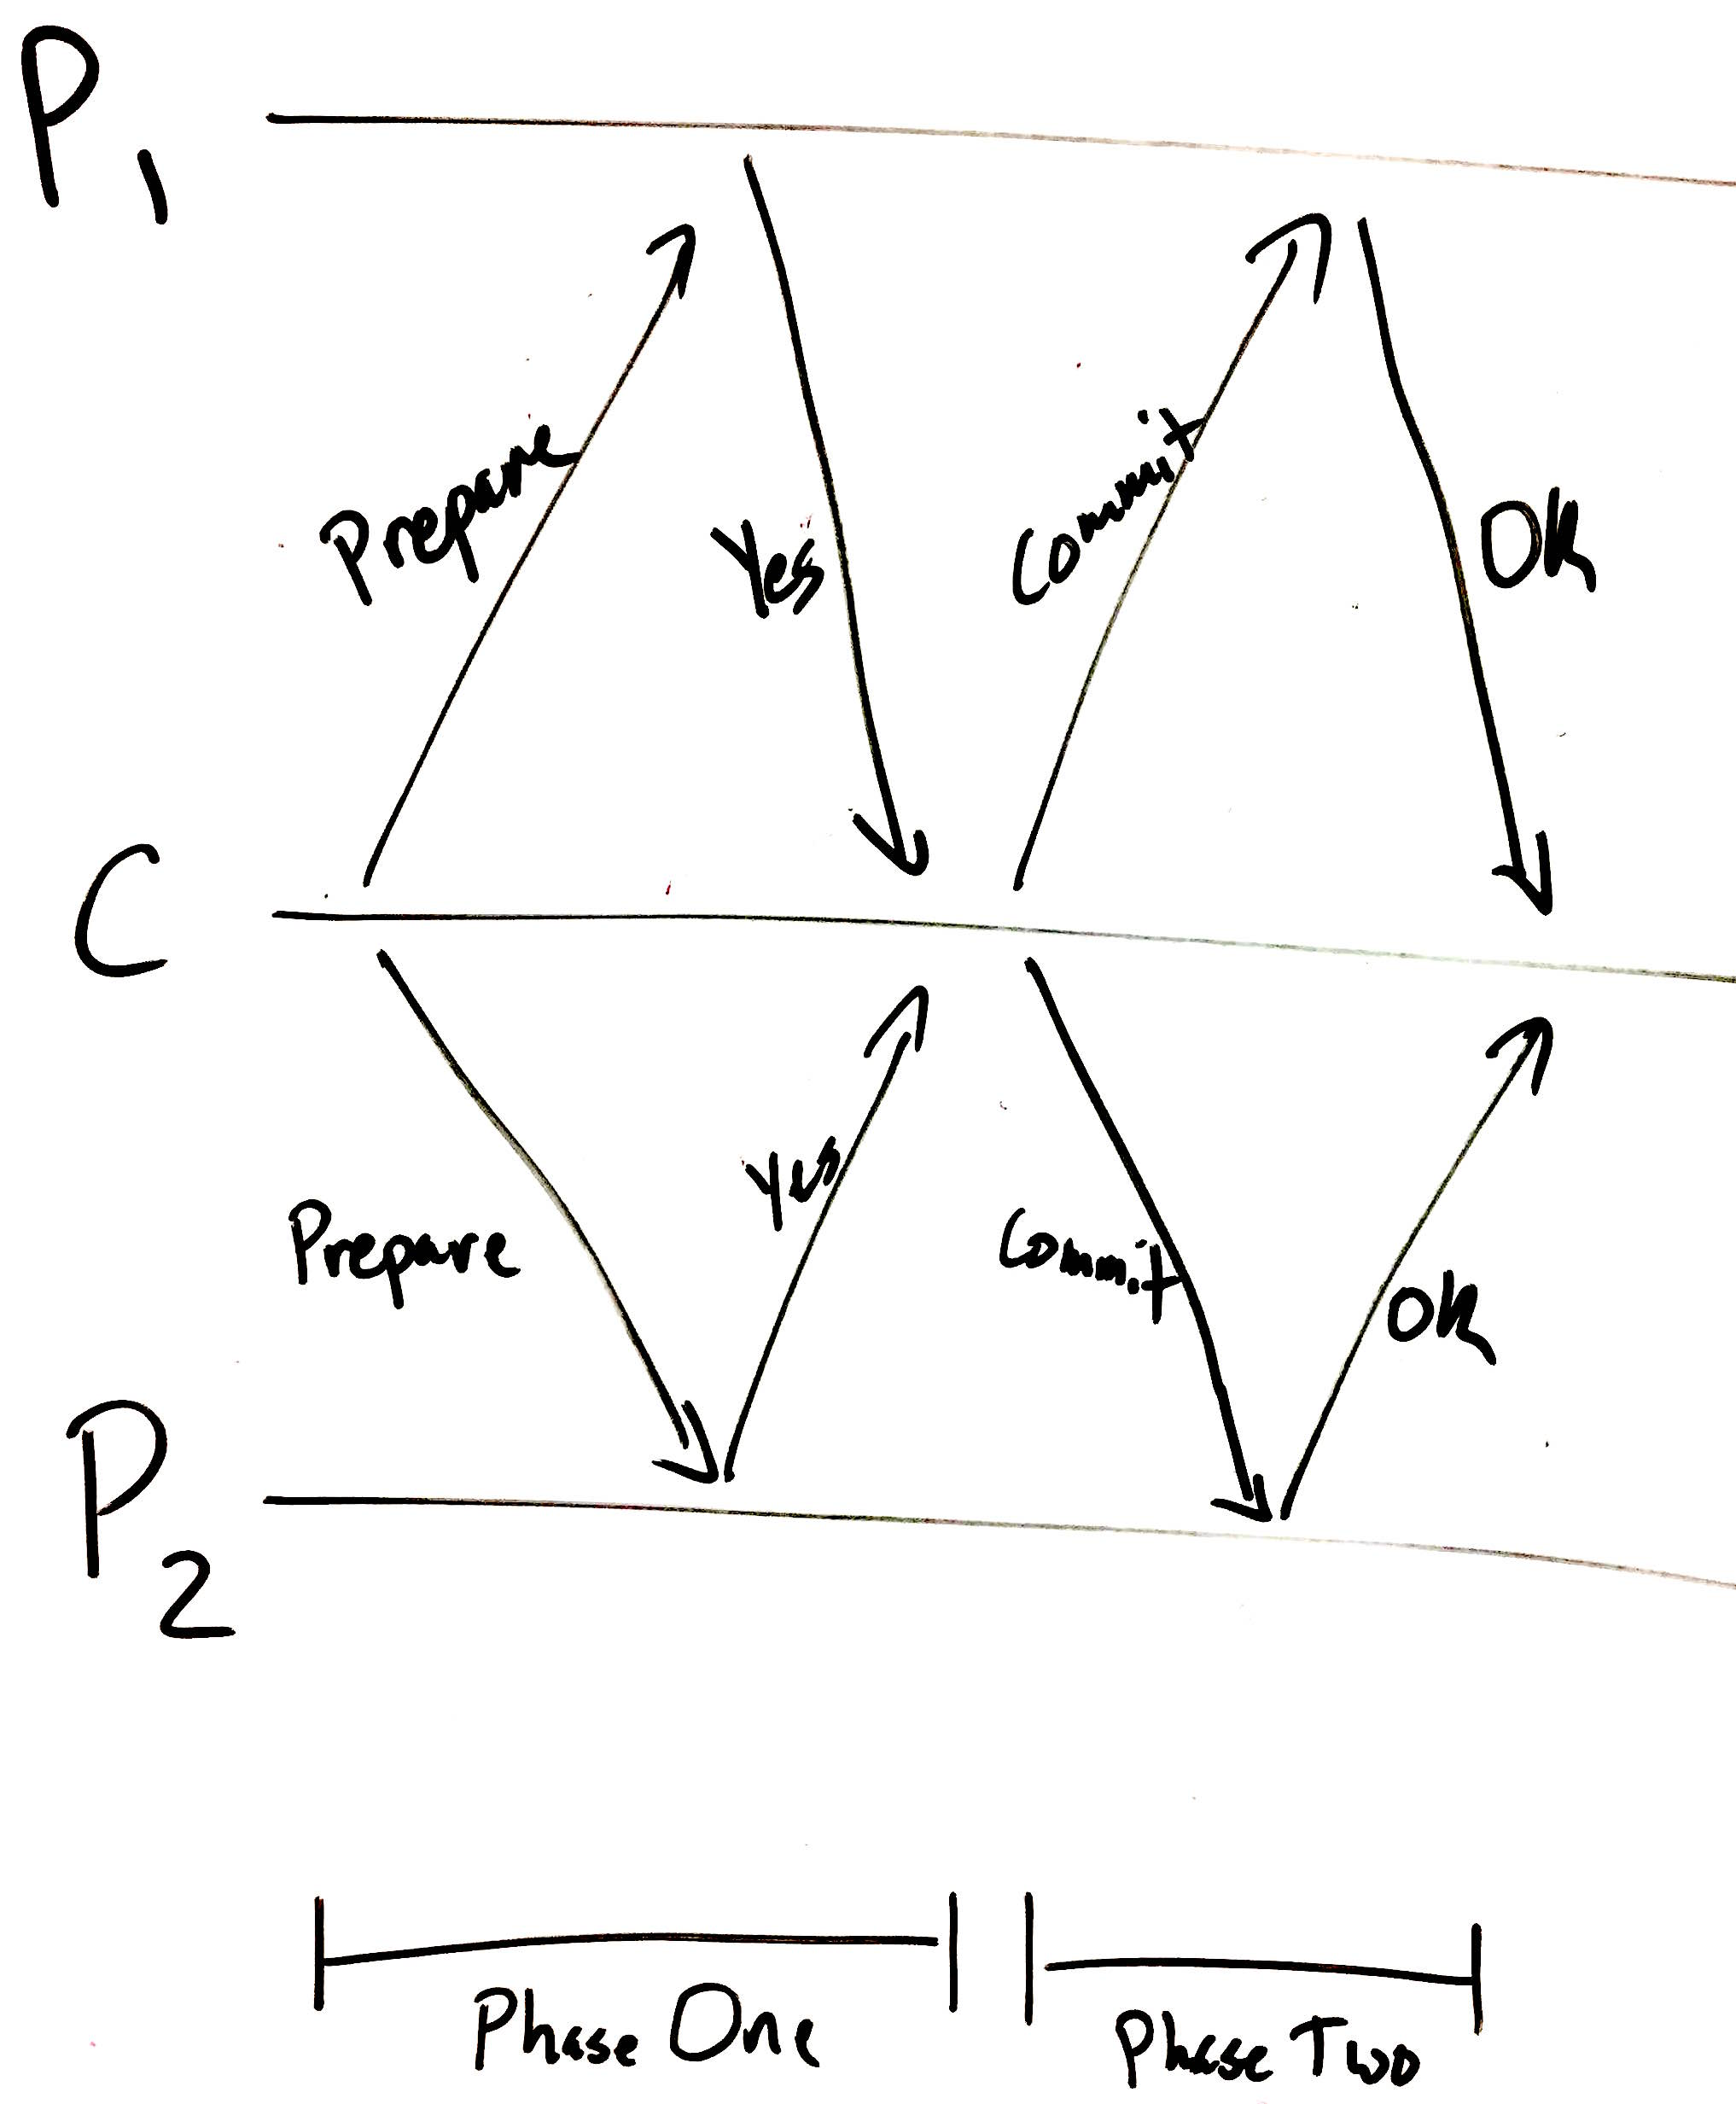
\includegraphics[width=0.96\textwidth]{tpc.pdf}
 \caption{One round of the Two-Phase Commit.}
  \label{fig:tpc-execution}
\end{minipage}
&
\begin{minipage}{0.55\linewidth}
\centering
\includegraphics[width=1.0\textwidth]{tpcstate.pdf}
\caption{States of a coordinator~(a) and a participant~(b).}
\label{fig:tpc-state}
\end{minipage}
\end{tabular}
\end{figure}
}




The Two-Phase Commit protocol designates a single node as the
\emph{coordinator}, which is in charge of managing the commit process;
other nodes participating in the protocol are \emph{participants}.
%
The protocol proceeds in a series of rounds, each of which makes a
single decision.
%
Each round consists of two phases; an example round execution is
shown in \cref{fig:tpc-execution}.
%
In phase one, the coordinator begins processing a new transaction by sending
$\tprep$ messages to all participants.
%
Each participant responds with its local decision $\tyes$ or $\tno$.
%
In the figure, both participants vote $\tyes$, so the coordinator
enters phase two by sending $\tcommit$ messages to all participants,
informing them of its decision to commit.
%
If some participant had voted $\tno$, the coordinator would instead
send $\tabort$ messages.
%
In either case, participants acknowledge the decision by sending
$\tackcommit$ or $\tackabort$ to the coordinator.
%
When the coordinator receives all acknowledgments, it knows that all
nodes have completed the transaction.

The component of the coherence predicate constraining the local state
\code{l} (expressed via Coq/Ssreflect predicate notation \code{[Pred l
  | ...]}) of each node \code{n} depending on its role, coordinator or
a participant, is defined as follows:

%\newpage

\begin{lstlisting}[style=Coq, basicstyle=\footnotesize\ttfamily]
Definition localCoh (n: nid) := [Pred l |
  if n == cn then exists(r: round) (s: CState) (log: Log), l = st :-> (r, s) \+ lg :-> log
  else if n \in pts
        then exists(r: round) (s: PState) (log: Log), l = st :-> (r, s) \+ lg :-> log else True].
\end{lstlisting}
%
%
According to the predicate \code{localCoh}, the local state of the
coordinator (\code{cn} is a parameter bound at the level of the
protocol description) consists of two globally defined locations,
\code{st} and \code{lg}, which together store a round number
\texttt{r}, a \emph{coordinator status} \texttt{s}, and a
\texttt{log}.
%
The state of a participant (\code{n} $\in$ \code{pts}) is similar, except
that its status is a \emph{participant status}.
%
Finally, any node which is not the coordinator or a participant (\eg,
a node participating only in other protocols) may have an arbitrary
local state with respect to \code{TPC}.

The coordinator's status can be in any of the seven states shown in
shown in \cref{fig:tpc-state}(a).
%
Between rounds, the coordinator waits in the $\cinit$ state.
%
From the initial state, the coordinators enters the \textsf{CSentPrep}
phase and remains in it until all prepare-requests are sent, after
which it switches into the receiving state $\mathsf{CWaitPrepResp}~x$
for the data $x$.
%
Upon receiving all response message to the prepare-requests, the
coordinator changes either to the commit-state or to the abort-state,
notifying all of the participants about the decision and collecting
the acknowledgements, eventually returning to the $\cinit$ state with
an updated log.
%
The participants follow a similar pattern to the coordinators's,
except that a participant sends messages to or receives messages
from only the coordinator before changing its state.

{
\begin{figure}[t!]
\setlength{\belowcaptionskip}{-10pt}
{\centering
\begin{tabular}{c@{\ }c}
\begin{minipage}{0.5\linewidth}
\begin{lstlisting}[style=Coq, basicstyle=\scriptsize\ttfamily]
Definition c_send_step (r: round) (cs: CState)
           (log: Log) (to: node) := match cs with
  (* Sending prepare-messages *)
  | CSentPrep x tos => if (* sent all messages *)
        (* switch for receiving responses *)
        then (r, CWaitPrepResp x [::], l)
        (* keep sending requests *)
        else (r, CSentPrep x (to :: tos), l)
  (* ...more cases depending on cs and to... *)
  end.



\end{lstlisting}
\end{minipage}
&
\begin{minipage}{0.5\linewidth}
\begin{lstlisting}[style=Coq, basicstyle=\scriptsize\ttfamily]
Definition c_recv_step (r : round) (cs : CState)
       (log : Log) (tag : nat) (mbody : seq nat) :=
  match cs with
  (* Waiting for prepare-responses *)
  | CWaitPrepResp x => if (* received all votes *)
      then (r, if (* all votes yes *)
                then CCommit x
	             else CAbort x, log)
      else (r, CWaitPrepResp, log)
  (* ...more cases depending on cs, tag, mbody... *)
  end.
\end{lstlisting}
\vspace{-8pt}
\end{minipage}
\end{tabular}
}
\caption{Send and receive transitions of a coordinator in a \disel
  definition of the {\small\texttt{{TPC}}} protocol.}
\label{fig:coordinator-trans}
\end{figure}
}

\Cref{fig:coordinator-trans} shows how to encode a few of the
coordinator's transitions.
%
Recall that \disel transitions are computable functions that describe
how to update the local state of the node when executing the
transition.
%
The figure shows the snippets of \disel code related to sending a
prepare-request messages and receiving a corresponding response
message from participants.
%
In the latter case, depending on the responses, once all of them are
collected, the coordinator switches to either \textsf{CCommit} or
\textsf{CAbort} state.


\subsection{Program Specification and Implementation}
\label{sec:tpc-impl}

With the protocol in hand, we can now proceed to build programs that
implement the coordinator and participant and assign them useful
Hoare-style specifications.
%
An implementation of a single round of the coordinator and its Hoare
type are shown in \cref{fig:tpc-ccode}.
%
The function \code{coordinator_round} takes as an argument the
transaction data to be processed in this round.
%
The type \code{\{r\ log\} DHT [cn, TPC] (...)} represents a Hoare
spec, whose logical variables are \code{r} and \code{log}. The spec is
parameterized by the dedicated coordinator node id \code{cn} and a
world with a single protocol instance \code{TPC}, with no hooks.
%
The pre/postconditions (in parentheses) are encoded as Coq functions
\code{fun s => ...} and \code{fun res s' => ...}, correspondingly, so
the immediate pre/post-states \code{s}/\code{s'} are made explicit,
similarly to using the connective $\This{\mathsf{s}}$.

The precondition, which makes use of the \emph{local state getter}
\code{loc cn s = ...}, equivalent to the connective
$\mathsf{cn} \ppts{\mathtt{TPC}} \ldots$ from \cref{fig:dsem},
requires that the coordinator is in the $\cinit$ state, with an
arbitrary round number and log.
%
The postcondition ensures that the local state has returned to
$\cinit$, the round number has been incremented, and the return value
accurately reflects the decision made on the data, which is also
reflected in the updated log.
%
The code proceeds along the lines required by the protocol: it reads
the round number from the local state, sends requests, collects the
responses and then, depending on the locally stored result~\texttt{b},
sends commit/abort messages, collecting the acknowledgements from
participants.

\subsection{Protocol Consistency and Inductive Invariant}
\label{sec:cons-induct-invar}

The spec given to \code{coordinator_round} in \cref{fig:tpc-ccode}
only constrains the local state \code{loc} of the coordinator, but
in fact the protocol maintains stronger global invariants.
%
For example, we might like to conclude that between rounds, all logs
are in agreement.
%
This strong global agreement property is not implied by the coherence
predicate given above, so we must prove an inductive invariant that
implies it.
%
Finding such inductive invariants is the art of verification, and the
process typically requires several iterations before converging on a
property that is inductive and implies the desired spec.
%
Tools such as Ivy~\cite{Padon-al:PLDI16} and \mypyvy~(\cref{chap:mypyvy}) make the process of finding
an inductive invariant much more pleasant by providing automatic
assistance in debugging and correcting invariants, or even inferring invariants automatically.
%
For now, though, we proceed to manually construct an invariant.

{
\setlength{\belowcaptionskip}{-10pt}
\begin{figure}
\centering
\begin{tabular}{@{\!\!}c@{\ }c}
\begin{minipage}{0.5\linewidth}
\begin{lstlisting}[style=Coq, basicstyle=\scriptsize\ttfamily]
Definition coordinator_round (d : data) :
{r log}, DHT [cn, TPC]
(fun s => loc cn s = st :-> (r, CInit) \+ lg :-> log,
 fun res s' =>
 loc cn s' = st:->(r+1, CInit) \+ lg:->(log++[(res, d)]))
  := Do (r <-- read_round;
         send_prep_loop r d;;
         res <-- receive_prep_loop r;
         b <-- read_resp_result;
         (if b then send_commits r d;;
                     receive_commit_loop r
                else send_aborts r d;;
                     receive_abort_loop r);;
           return b).
\end{lstlisting}
\vspace{-10pt}
\caption{Spec and code of a coordinator round.}
\label{fig:tpc-ccode}
\end{minipage}
&
\setlength{\belowcaptionskip}{-10pt}
\begin{minipage}{0.5\linewidth}
\begin{lstlisting}[style=Coq, basicstyle=\scriptsize\ttfamily]
Definition run_coordinator (data_seq : seq data) :
DHT [cn, _]
(fun s => s = loc cn s = st :-> (0, CInit) \+ lg :-> [::]
 fun _ s' => exists (choices : seq bool),
   let r  := size data_seq in
   let lg := zip choices data_seq in
   loc cn s' = st :-> (r, CInit) \+ lg :-> log /\
   forall pt, pt \in pts ->
         loc pt s' = st :-> (r, PInit) \+ lg :-> log)
 := Do (with_inv TPCInv (coordinator data_seq)).
\end{lstlisting}
\vspace{25pt}
\caption{Coordinator spec elaborated with {\small\texttt{{TPCInv}}}.}
\label{fig:tpc-with-inv}
\end{minipage}
\end{tabular}
\end{figure}
}



% \begin{figure}[t]
% {\centering
% \begin{lstlisting}[style=Coq, basicstyle=\footnotesize\ttfamily]
% Definition pt_PhaseTwoCommit cn pt r x log ms :=
% (loc pt = st :-> (r, PRespYes x) \+ lg :-> log
%  /\$ $ msg_spec cn pt commit_req [r] ms
%  /\$ $ no_msg_from_to pt cn ms) \/
% (loc pt = st:-> (r, PCommitted x) \+$\!$ lg :-> (log++[(true, x)])
%  /\$ $ no_msg_from_to cn pt ms
%  /\$ $ no_msg_from_to pt cn ms) \/
% (st :-> (r + 1, PInit) \+ lg :-> (log ++ [(true, x)])
%  /\$ $ no_msg_from_to cn pt ms
%  /\$ $ msg_spec pt cn commit_ack [r] ms).
% \end{lstlisting}
% }
% \caption{Part of the inductive invariant for a participant \texttt{pt}, describing the second phase after \texttt{pt} agreed to commit.}
% \label{fig:tpc-inv}
% \end{figure}

In this case, an invariant that closely follows the intuitive
execution of the protocol (its formulation can be found in our Coq
files) suffices to prove the global log agreement property.
%
For example, when the coordinator is in the $\csendcommit$ state, the
invariant ensures that all participants are either waiting to hear
about the decision, have received the decision but not acknowledged
it, or have acknowledged the decision and returned to the initial state.
%
The invariant also implies a simple statement of \emph{global log agreement},
shown below:
%
\begin{lstlisting}[style=Coq, basicstyle=\footnotesize\ttfamily]
Lemma cn_log_agreement d r log pt : loc cn d = st :-> (r, CInit) \+ lg :-> log ->
        coh d -> TPCInv d -> forall pt, pt \in pts -> loc pt d = st :-> (r, PInit) \+ lg :-> log.
\end{lstlisting}
%
In other words, a coordinator \code{cn} in the $\cinit$ state and a
round \code{r} can conclude that \emph{all} participants
{\small{$\mathtt{pt} \in \mathtt{pts}$}} have also reached the current
round \code{r} and have logs equal to its own.

\paragraph{Putting the inductive invariant to work.~}

We can freely use the elaborated invariant in proofs of programs.
%
\Cref{fig:tpc-with-inv} shows a coordinator program that executes
a series of rounds based on a given list \code{data_seq} of data
elements.
%
Its postcondition asserts that all participants have finished the
round and have logs agreeing with the one of the coordinator.
%
The proof of this specification is by a straightforward application of
the \textsc{WithInv} rule, making use of the elaborated invariant
\code{TPCInv} as well as the lemma \code{cn_log_agreement}.
%
Importantly, the postcondition is stable, because each round of the
Two-Phase Commit begins with a coordinator's move, hence no
participant can change its state from the ``initial'' one while the
coordinator's status is~$\cinit$.

\subsection{Composing Two-Phase Commit with a Querying Application
  using Hooks}
\label{sec:composing-two-phase}


Even though core consensus protocols, such as \code{TPC}, are not
designed to exist in isolation, but rather to be used in a context of
larger applications (\eg, for crash recovery), formal reasoning about
\emph{client-specific properties} (\ie, properties of applications
relying on certain characteristics of a ``core'' distributed protocol) is only
barely covered in classical textbooks~\cite{Weikum-Vossen:TIS02} and,
with a rare exception~\cite{Lesani-al:POPL16}, almost never a focus of
major verification
efforts~\cite{Woos-al:CPP16,Hawblitzel-al:SOSP15,rahli:eventml-avocs},
which, therefore cannot be reused in any larger verified context.

We now demonstrate how to employ \disel's logical mechanisms for
restricted composition of protocols in order to prove, in a modular
fashion, properties of client code from a core protocol's invariants.
%
To do so, we verify a composite application, which uses \code{TPC} for
building a replicated log of data elements, and a \emph{side-channel
  protocol} for sending independent queries about the state of
\code{TPC} participants (\eg, for the purpose of implementing recovery
after a coordinator's failure).
%
\Cref{fig:cn-query} shows a program that first calls the
coordinator program \code{run_coordinator}, and then uses the side
protocol to query the local state of a participant \code{pt}, which
the program then returns as its final result \code{res}.  Ignoring the
\code{query_init} part in the pre/postcondition for now, notice that
the postcondition asserts that \code{res} is \emph{equal to} the pair
\code{d} (round, log) stored in the local state of the coordinator
(which did not crash this time)!

Establishing such validity of the query \wrt \code{TPC}-related state
is, however, not trivial at all, given how the querying protocol is
defined. The protocol \code{Query} is very similar to the calculator
from \cref{sec:overview}: any node $n_1$ in it can send a
request to any other node $n_2$, to which $n_2$ may respond with
\emph{any} arbitrary message (the details of the formal protocol
definition can be found in our Coq code). This protocol definition is
intentionally made very weak: while it allows one to prove some
interesting inductive invariants (\eg, no request is answered twice),
it leaves all other interaction aspects for the final client to
specify. In particular, it \emph{does not} enforce any specific shape
of data being sent in a response to a request.

{
\setlength{\belowcaptionskip}{-10pt}
\begin{figure}
\centering
\begin{tabular}{c@{\ }c}
\!\!\!\!
\begin{minipage}{0.5\linewidth}
\begin{lstlisting}[style=Coq, basicstyle=\scriptsize\ttfamily]
Program Definition run_and_query (ds : seq data) pt :
  {reqs resp}, DHT [cn, (TPC \+ Query, QHook)]
  (fun s => loc s = st :-> (0, CInit) \+ lg :-> [::] /\
             pt \in pts  $\aand$  query_init s],
   fun (res : nat * Log) s' => exists (chs : seq bool),
     let d := (size ds, zip chs ds) in
     loc s' = st :-> (d.1, CInit) \+ lg :-> d.2 /\
     query_init s' $\aand$ res = d)
  := Do (run_coordinator ds;;
          rid <-- generate_fresh_request_id pt;
          send_request rid pt;;
          res <-- receive_responce rid pt;
          return res).
\end{lstlisting}
\vspace{18pt}
\caption{Querying after the {\small\texttt{TPC}} coordinator.}
\label{fig:cn-query}
\end{minipage}
&
\begin{minipage}{0.5\linewidth}
\begin{lstlisting}[style=Coq, basicstyle=\scriptsize\ttfamily]
Parameter core_state : Data -> LocState -> Prop.
Parameter local_indicator : Data -> LocState -> Prop.

Definition QHook := (1, lab_c, lab_q, resp) :->
 fun lc lq m to =>
 forall rid data, m = rid :: serialize data ->
               core_state data lc.

Hypothesis core_state_inj :
  forall l d d', core_state d l ->
             core_state d' l -> d = d'.

Hypothesis core_state_step : forall data s s' n1 n2,
  n1 != n2 -> local_indicator data (loc lab_c n1 s)
  -> network_step (lab_c :-> pc, $\emptyset$) n2 s s'
  -> core_state data (loc lab_c n2 s').
\end{lstlisting}
\vspace{-10pt}

\caption{Hook definition and abstract predicates.}
\label{fig:hook-ap}
\end{minipage}
\end{tabular}
\end{figure}
}


Thus, without imposing the additional restriction that the protocol
\code{Query} \emph{can only transmit the local state of a node} \wrt
\code{TPC}, we will not be able to prove the spec in
\cref{fig:cn-query}.
%
%This is where the mechanism of \disel's send-hooks comes to rescue.
%
The necessary restriction is provided by a send-hook entry
\code{QHook} that is used when composing the protocols \code{TPC} and
\code{Query} in the spec of \code{run_and_query}, and is defined in
\cref{fig:hook-ap}.

In order to make the client verification effort reusable in the
context of \emph{any} consensus protocol, not just \code{TPC}, we
formulate the hook statement in terms of an abstract type \code{Data}
and an \emph{abstract predicate} \code{core_state}, which we will
later instantiate specifically for \code{TPC}, both afforded by Coq's
higher-order programming capabilities. The hook enforces that any
message \code{m} containing a request id \code{rid} and serialized
\code{data} adequately encodes the current local state (storing
\code{data}) of the sender node, at the moment of sending~\code{m},
with respect to the protocol with label \code{lab_c}.
%
The abstract predicate \code{core_state d lc}, capturing precisely
this ``adequacy of the encoding'', is supplied with the injectivity
hypothesis \code{core_state_inj} (to be proved by each consensus
implementation), which ensures that the abstract data representation
is unambiguous.

We also declare an abstract predicate \code{local_indicator} and the
corresponding hypothesis \code{core_state_step}, which essentially
corresponds to \emph{irrevocability} of consensus and should be proved
for each consensus implementation (in particular, for \code{TPC}),
ensuring that if a local state of a node \code{n1} is of certain shape
\code{data}, the local state of \code{n2}, captured by
\code{core_state data} will be remaining \emph{the same} under
interference (\code{network_step}) \wrt the core \code{lab_c}-labelled
protocol~\code{pc}---precisely what is ensured by the lemma
\code{cn_log_agreement} of~\code{TPC}.

Finally, we can use the abstract predicates from
\cref{fig:hook-ap} to provide specifications for querying
procedures from \cref{fig:cn-query}, stating \code{query_init} in
terms of assertions involving \code{local_indicator} and
\code{query_state}, in the context \emph{parameterized} over a
``core'' consensus protocol \code{pc} and restricted with
\code{QHook}.
%
To verify the program in \cref{fig:cn-query} against the desired
spec we only need to instantiate the predicates as follows and prove
the corresponding hypotheses for \code{TPC}, which follow from the
invariant \code{TPCInv} and Lemma~\code{cn_log_agreement}:

\begin{lstlisting}[style=Coq, basicstyle=\footnotesize\ttfamily]
(* For TPC, abstract Data type is instantiated with a round number (nat) and Log. *)
Definition Data := nat * Log.
Definition local_indicator (d : Data) l := l = st :-> (d.1, CInit) \+ log :-> d.2.
Definition core_state (d : Data) l        := l = st :-> (d.1, PInit) \+ log :-> d.2.
\end{lstlisting}
%
The rest of the proof is via the \Rule{Frame} rule with
$W = \angled{\text{\code{TPC}}, \emptyset}$, $C = \text{\code{Query}}$ and
$H = \text{\code{QHook}}$. Since \code{QHook} does not restrict the
transitions of \code{TPC}, $\NHooked$ holds.
%
Thanks to the parameterization of querying programs with abstract
predicates and hypotheses from \cref{fig:hook-ap}, we can compose
them with any other instance of a consensus protocol, \eg,
Paxos~\cite{Lamport:TOPLAS98} or Raft~\cite{ongaro:raft},
thus, reusing the proofs of their core invariants.

\section{Implementation and Experience}
\label{sec:eval-impl}

\disel combines two traits that rarely occur in a single tool for
reasoning about programs.  First, thanks to the representation of Hoare
types by means of Coq's dependent types, the soundness result of
\disel scales not just to a toy core calculus, but to the entirety of
Gallina, the \emph{programming language} of Coq, enhanced with general
recursion and message-passing primitives.
%
Second, \disel programs are immediately \emph{executable} by means of
extracting them into OCaml, which provides the features that Gallina
lacks: general fixpoints, mutable state, and networking constructs,
enabled by our trusted shim implementation.

% We briefly outline our experience of conducting mechanized proofs in
% \disel, and elaborate on some technical insights \wrt implementing an
% extraction mechanism for verified distributed programs with a minimal
% trusted code base.

\paragraph{Formal development and proof sizes.~}
%
The size of our formalization of the metatheory, inference rules and
soundness proofs is about 4500 LOC.  Our development builds on
well-established {Ssreflect}/MathComp libraries
\cite{Gonthier-al:TR,Maboubi-Tassi:MathComp,Sergey:PnP} as well as on
the implementation of partial finite maps and heap theory
by~\citet{Nanevski-al:POPL10}.

%
\begin{table}[t]
\centering
\begin{minipage}{0.54\textwidth}
{
\sffamily\footnotesize
% \centering
%\vspace{-12pt}
\begin{tabular}{|l|c|c|c|c|}
\hline
{Component} &
{ {Defs/Specs}} & {{Impl}} & {{Proofs}} &
{Build}
\\ \hline \hline
% \multicolumn{6}{|c|}{\textbf{Greeter}} \\\hline
% \emph{protocol} & 95& - & 40 & \multirow{2}{*}{2.5} & \multirow{2}{*}{$<$0.5\!}\\
% \textsf{hello\_world} &60 & 8 &78 & &  \\\hline
  \multicolumn{5}{|c|}{\textbf{Calculator} (\S\ref{sec:overview})} \\\hline
  \emph{protocol} (\S\ref{sec:calc-prot}) & \multirow{3}{*}{239} &
        \multirow{3}{*}{-} & \multirow{3}{*}{243} &\multirow{3}{*}{4.8}  \\
  $\Inv_1$ (\S\ref{sec:elab-calc}) &&&& \\
  $\Inv_2$ (\S\ref{sec:more-impl-free}) &&&& \\\hline
  \textsf{$\osserver$} (\S\ref{sec:elab-calc}) & \multirow{3}{*}{192}
                & \multirow{3}{*}{43} & \multirow{3}{*}{153} &
                                                               \multirow{3}{*}{8.6} \\
  \textsf{$\bserver$} (\S\ref{sec:more-impl-free}) &&&& \\
  \textsf{$\mserver$} (\S\ref{sec:more-impl-free}) &&&& \\\hline
  \textsf{$\cclient$} (\S\ref{sec:more-impl-free}) & 120 & 24 & 99 & 4.8 \\
  \textsf{$\dserver$} (\S\ref{sec:more-impl-free}) & 75 & 7 & 49 &2.4 \\\hline
  \multicolumn{5}{|c|}{\textbf{Two-Phase Commit}
  (\S\ref{sec:tpc-prot}--\S\ref{sec:cons-induct-invar})}
  \\\hline
  \emph{protocol} (\S\ref{sec:tpc-prot}) & 465 & - & 231 & 3.9 \\\hline
  \textsf{coordinator} (\S\ref{sec:tpc-impl}) & 236  &  35  & 440 & 18 \\\hline
  \textsf{participant} (\S\ref{sec:tpc-impl}) & 163 & 24 & 198 & 10 \\\hline
  \texttt{\TPCInv} (\S\ref{sec:cons-induct-invar}) & 997 & - & 2113 & 25 \\\hline
  %
  \multicolumn{5}{|c|}{\textbf{{Query}/{TPC}} (\S\ref{sec:composing-two-phase})} \\\hline
  \emph{protocol} & 169 & - & 115 & 2.1 \\\hline
  querying procedures & 326  &  18  & 707 & 19 \\\hline
  {\small\texttt{run\_and\_query}} & 76 & 5 & 89 & 2.6 \\
  %
  [2pt]\hline
\end{tabular}
\vspace{5pt}
}
\end{minipage}
\caption{Statistics for implemented systems: sizes of protocol
  definitions/specs, programs, proofs of protocol
  axioms/invariants/specs (LOC), and build times (sec).  }
\label{tab:locs}
\end{table}
%
Table~\ref{tab:locs} summarizes the proof effort for the calculator,
\code{TPC}/\code{Query} systems.
%
The \textsf{Defs/Specs} column measures all \emph{specification}
components, including, \eg, auxiliary predicates, whereas
\textsf{Impl} reports the sizes of actual \disel programs.
%
Due to the high degree of code reuse, it is difficult to provide
separate metrics in some cases; for those parts we only report the
joint numbers.
%
Although \disel is not yet a production-quality verification tool,
safety proofs of interesting systems can be obtained in it in a
reasonably short period of time and with moderate verification effort
(\eg, the full development of the core \code{TPC} system took nine
person-days of work).
%
Given that the current version of \disel employs no advanced proof
automation, beyond what is offered by Coq/Ssreflect, for discharging
program-level verification conditions~\cite{chlipala:bedrock} or
inductive invariant proofs~\cite{Padon-al:PLDI16}, we consider these
results encouraging for future development.

\paragraph{Extraction and execution.~}
\label{sec:extracting-runtime}

\disel's logic reasons about programs in terms of their denotational
semantics as traces, but each primitive also has a
straightforward operational meaning.
%
For example, executing a wrapped send transition should actually send
the corresponding network message.
%
Thus it is relatively straightforward to extract \disel programs by
providing OCaml implementations of the primitive operations in a
trusted shim.
%
Our shim consists of about 250 lines of OCaml, including primitives
for sending and receiving messages and general recursion.
%
The local state of each node is implemented as a map from protocol
labels to heaps, where a heap is implemented as a map from locations
to values.
%
Since \disel does not draw a distinction between real and auxiliary
state so far, both are manifested at run time.
%
In the future, we plan to allow users to mark state as auxiliary to
improve performance.
%
Due to artifacts of the extraction process, a \disel program that
appears tail-recursive at the Coq source level does not extract to a
tail-recursive OCaml program.
%
This causes long running loops (such as those typically used to
implement blocking receive) to quickly blow the OCaml stack.
%
To circumvent this issue, we added a while-loop combinator to \disel,
which is encoded using the general fixpoint combinator, but is extracted to
an efficient OCaml procedure that uses constant stack space.
%
Our implementations of the calculator and \code{TPC} use this
while-loop combinator to implement blocking receive.
%

In this work, our goal was not to extract high-performance code for
\disel programs, but rather show that, with a careful choice of
low-level primitives with precise operational meaning, such extraction
is feasible and requires a very small trusted codebase.
%
% We leave generation of fast distributed code (\eg, via
% staging~\cite{Romp:WF16}) for future work.

\paragraph{Adequacy of the extraction.~}

What is the correspondence between our denotational semantics,
presented in \cref{sec:soundness} and the operational one
implemented by our shim?
%
% Understanding this relation important in order to gain confidence in
% the resulting system.
%
While in this work we do not state a fully formal correspondence, as
the shim is written in OCaml and uses operating system and network
components, which have no formal semantics, we argue that the
extraction is adequate \wrt the denotational semantics for the
following reasons:

\begin{enumerate}

\item Our denotational semantics is simply a trace-collecting
  operational semantics for interleaved, asynchronous, message-passing
  concurrency, with the shared message soup being the only
  communication medium. Such an operational representation is widely
  considered adequate for modelling distributed systems and has been
  employed and evaluated (also, without verifying the extraction) in
  previous works~\cite{
    Wilcox-al:PLDI15,Hawblitzel-al:SOSP15,Padon-al:PLDI16}.

\item The shim implementation follows the operational rules from
  \cref{fig:nsem} verbatim, and protocol transitions are encoded
  in \disel as \emph{functions} on the local state, so they are easy
  to extract and execute. The shim, thus, provides an accurate
  implementation of the protocol-aware network semantics.

\end{enumerate}

\noindent
%
Our fixpoint definition (available in our Coq sources) admits
non-terminating executions, ``approximating'' them iteratively by sets
of incomplete post-safe traces. It is extracted into OCaml's general
fixpoint operator, with a somewhat ad hoc tail-call optimisation
described above in this Section. This means that our logic proves only
partial correctness: verified programs may loop at runtime, but they
will never violate the protocol.

\paragraph{Information hiding and separation.~}

One might wonder whether we can \emph{hide} implementation-specific
parts of local state from the clients, \eg, when reasoning about other
nodes' implementations?
%
At the moment any mutable state in \disel should be manifested
\emph{in a protocol definition} (and, thus, \emph{known} to all its
users) and can be only altered by sending/receiving. This is why in
the examples, such as the memoizing calculator from
\cref{sec:more-impl-free}, we model hidden state by passing a
functional argument. However, what the framework \emph{does allow} one
to do is to encode an auxiliary protocol implementing a mutable
storage, which, once joined (via~$\uplus$) with its client protocol
(\eg, calculator), \emph{does not} have to be exposed to the clients
of the latter one, similarly to how it is done in the delegating
calculator example.

To support a version of a ``proper'' hidden local mutable state (\ie,
a heap with mutable pointers) we would need to formulate a nested
program logic with the corresponding low-level semantics for
state-manipulating programs---a direction we consider as interesting
future work, with an idea of adopting for this role Verifiable~C
by~\citet{Appel-al:BOOK14}.


\section{Related and Future Work}
\label{sec:related}

\subsection{Program Logics for Concurrency}

\disel builds on many ideas from modern program logics for
compositional concurrency reasoning.
%
The notion of protocols (often called \emph{regions}) in shared-memory
concurrency
logics~\cite{Turon-al:POPL13,DinsdaleYoung-al:ECOOP10,Nanevski-al:ESOP14,Turon-al:OOPSLA14,Raad-al:ESOP15,Svendsen-Birkedal:ESOP14}
provides a ``localized'' version of more traditional Rely/Guarantee
obligations~\cite{Jones:TOPLAS83}, which, in their original
formulation, are not
modular~\cite{Vafeiadis-Parkinson:CONCUR07,Feng:POPL09,Feng-al:ESOP07}.
%
The two closest to \disel logics employing protocols to reason about
interference are FCSL by~\citet{Nanevski-al:ESOP14} and GPS
by~\citet{Turon-al:OOPSLA14}. Besides those being logics for
\emph{shared-memory}, rather than \emph{message-passing} concurrency,
protocols in FCSL and GPS are tailored for the notion of
\emph{ownership transfer}~\cite{OHearn:TCS07}, as a way to express
exclusivity of access to shared resources.
%
Due to the lack of \emph{immediate} synchronization between nodes in a
message-passing setting, we consider the notion of ownership to be of
less use for most of the systems of interest. That said, even though
\disel does not feature explicit ownership transfer, it can be easily
encoded on a per-protocol basis, by defining a suitable local state
and transitions.

Composition of modular proofs about protocols is a problem that has
not received much attention in modern concurrency logics. In FCSL,
which tackles a similar challenge, in order to constrain
inter-protocol interaction, a user must set up her protocols with a
very specific foresight of how they are going to be composed with
other protocols, defining \emph{intrinsic} ``ownership communication
channels'' for \emph{all} involved components, thus, effectively
prohibiting unforeseen interaction scenarios. This is not the case in
\disel: as we have shown in \cref{sec:tpc}, ``core'' and
``client'' protocols (\eg, \code{TPC} and \code{Query}) can be
developed and verified independently and then composed in joint
applications via \emph{extrinsic} client-specified send-hooks.

The recent logical framework Iris~\cite{Jung-al:POPL15,Jung-al:ICFP16}
suggests to express protocols as a specific case of resources,
represented, in general, by partial commutative monoids, viewing
\emph{state reachability} as a specific instance of
\emph{framing}~\cite{Reynolds:LICS02}. This generality does not buy
much for verifying distributed applications, as the resulting proof
obligations are the same as when proving inductive invariants.  Having
an \emph{explicit} notion of protocols in the logic, though, allowed
us to provide the novel protocol-tailored rules \textsc{WithInv} and
\textsc{Frame} (\cf \cref{fig:semass}), which enabled modular
invariant proofs and distributed systems composition.

A related logic by~\citet{Villard-al:APLAS09} only considers protocols
associated with specific message-passing channels, rather than entire
distributed systems.
%
% that is, not allowing one to make global
% assertions about a system's state, which is necessary to specify, \eg,
% consistency properties of \code{TPC}.
%
In Villard~\etal's logic, messages do not carry any payload: they are
simply \emph{tags}, indicating ownership transfer of a certain heap
portion in the \emph{same} shared memory space. It is not immediately
obvious how to use Villard~\etal's specifications for \emph{locally}
asserting \emph{global} properties of stateful distributed systems
(e.g., the agreement of \code{TPC} in \cref{fig:tpc-with-inv})
without considering all involved processes.
%
In addition to that, Villard~\etal's logic does not provide a
mechanism for establishing inductive contract invariants.
%
A recent framework \emph{Actor Services}
by~\citet{Summers-Muller:ESOP16} provides abstractions similar to our
protocol transitions, but only allows to state \emph{local} actor
invariants, and lacks a formal metatheory and soundness proof.
%

To the best of our knowledge, none of the existing concurrency logics
features \emph{both} a foundational soundness proof (\ie, the proof that
the entire logic, not just its toy subset, is sound as a verification
tool), \emph{and} a mechanism to extract and run verified
applications.
%
% Furthermore, from the state-of-the art concurrency logics, only
% FCSL~\cite{Nanevski-al:ESOP14}, GPS~\cite{Turon-al:OOPSLA14} and
% Iris~\cite{Jung-al:POPL15} come with the foundational mechanized
% proofs of soundness, but those are logics for \emph{shared-memory}
% concurrency, rather than for message-passing distributed
% systems. Encoding the distributed message-based communication with the
% corresponding notion of distributed state, principles of modular
% reasoning and protocol composition in those logics, even if possible,
% is not trivial and has not been done yet.

\subsection{Types for Distributed Systems}
%
% A number of type systems have been proposed for distributed programs
% to enforce race-freedom and local state
% invariants~\cite{Kloos-al:ECOOP15}, ownership
% transfer~\cite{Haller-Odersky:ECOOP10},
% immutability~\cite{Liblit-Aiken:POPL00,Gordon-al:OOPSLA12}
% disciplines.
%
Session Types~\cite{Honda-al:ESOP98} are traditionally used to ensure
that distributed parties follow a predefined communication protocol
\wrt a specific channel. While the
\emph{multiparty}~\cite{Honda-al:POPL08} and
\emph{multirole}~\cite{Denielou-Yoshida:POPL11} Session Types enable a
form of system composition and role-play, and \emph{dependent session
  types} allow one to quantify over messages~\cite{Toninho-al:PPDP11},
session types do not allow quantification over the global system state
and reasoning out of inductive invariants, neither do they allow
restricted composition of protocols.

We believe that \disel's combination of Hoare types and protocols
provides the necessary level of expressivity to capture rich safety
properties of distributed applications.
%
A similar approach has been explored in $\fstar$
by~\citet{Swamy-al:ICFP11}, although that work did not reason about
inductive invariants separately from implementations, neither did it
address composition of systems with inter-protocol dependencies.

\subsection{Verification of Large Systems}

Recent work has verified implementations of core pieces of distributed
systems infrastructure, both by using specialized models and DSLs.


IronFleet~\cite{Hawblitzel-al:SOSP15} supports proving \emph{liveness}
in addition to safety, all embedded in Dafny~\cite{Leino:LPAR10}.
%
% Its Hoare logic fragment is \emph{local} and does not allow to
% quantify over global system state.
%
IronFleet focuses on layered verification of standalone monolithic
systems.
%
In those systems, each layer is a state-transition system (STS)
specifying the system's behavior at a certain abstraction level, with
the top-most layer expressing how a collection of nodes together
implement a high-level (\eg, shared-memory) specification,
%
and the actual implementation, run by the nodes, at the bottom.
%
Adjacent layers are connected by establishing refinement between
their %
STSs via reduction~\cite{Lipton-CACM75}, which often involves proving
inductive invariants, similar to what we have proven in \disel.
%
% IronFleet's specifications in the form of abstract STSs hide
% complexity of distributed interaction in a system, allowing the
% clients to reason about the system's properties.
%
In our understanding, such specifications do not allow for horizontal
composition, \ie, reasoning about interaction with separately verified
systems in a client code.
%
Such an interaction has been, however, explored \wrt
\emph{shared-memory} concurrency by~\citet{Gu-al:OSDI16}, who built a
series of abstraction layers in a verified concurrent OS kernel. That
work has shown that establishing a refinement between a spec STSs and
a \emph{family} of interacting lower-level STSs is possible, although
the proofs are usually quite complex, as they involve reasoning about
\emph{semantics} of a restricted product of STSs.
%
In contrast with those systems, \disel's logic does not provide
machinery to establish STS refinement, but rather explicitly
identifies valid linearization points~\cite{herlihy:linearizability} in
the implementations, as they correspond precisely to taken protocol
transitions.
%
Abstract specifications and the corresponding system properties, usable
by client code, such as consensus, are encoded in \disel via
parameterized Hoare types and abstract predicates, as shown in
\cref{sec:composing-two-phase}.

The Chapar framework by~\citet{Lesani-al:POPL16} is tailored to
causally consistent key-value stores, and also provides verified model
checking for client programs using the verified KV stores.
%
Ivy is a tool to assist users in iteratively discovering inductive
invariants by finding counterexamples to
induction~\cite{Padon-al:PLDI16}.
%
\textsc{PSync} by~\citet{Dragoi-al:POPL16} is a DSL allowing one to
prove inductive invariants of consensus algorithms in networks with
potential faults, operating in a synchronous round-based
model~\cite{Elrad-Frances:SCP82}. This assumption enables efficient
proof automation, but prohibits low-level optimizations, such as, \eg,
batching.
%
Mace by~\citet{killian:mace} and DistAlgo
by~\citet{Liu-al:OOPSLA12} adopt an asynchronous protocol model,
similar to ours.
%
Mace provides a suite of tools for generating and model checking
distributed systems, while DistAlgo allows extraction of efficient
implementation from a high-level protocol description.
%
EventML is another DSL for verifying monolithic distributed systems,
based on compiling to the Logic of Events in
Nuprl~\cite{rahli:eventml-avocs}.
%
None of these frameworks tackles the challenges of modular reasoning
about horizontally composed systems~\textbf{(2)} and elaborated
protocols~\textbf{(3)}, stated in the introduction of this chapter.

Arguably, our Two-Phase Commit implementation is a relatively small
case study when compared to the systems verified in Verdi (\cref{chap:verdi}) or in other frameworks including IronFleet and EventML.
Nevertheless, given enough time and effort, we are confident we could conduct safety proofs of
Raft~\cite{ongaro:raft} and
MultiPaxos~\cite{vanRenesse-Altinbuken:ACS15} in \disel, as their
implementations and invariants are based on the same semantic
primitives and reasoning principles that were employed for \code{TPC}.
%
We believe, though, that compositionality, afforded by \disel's
logical mechanisms, is a key to make the results of future
verification efforts reusable for building even larger verified
distributed ecosystems.

\section{Conclusion}

This chapter presented \disel,
  a concurrent separation logic for distributed systems.
\disel's key contribution to this dissertation is
  \emph{horizontal protocol composition},
  made possible by our frame rule, with hooks to express protocol dependencies.
We showed examples of composing protocols,
  including using two-phase commit mediate access to a distributed resource.
More generally, \disel allows us to compose separately designed and verified protocols
  to build more complex systems from existing pieces.
Together with the vertical decomposition provided by Verdi,
  one can systematically break down a large distributed system
  into independently verifiable protocols that add up to a verified whole.
